\chapter{A-Priori Reduction of Scenario Approximation for Dynamic DC-OPF}
This chapter is based on the publication of the dissertation author: \fullcite{lukashevich2023importance}. 
\label{chap:apriori_stochastic_approx}

\section{Introduction}
\label{sec:introduction}
\vspace{-1mm}
Integrating renewable energy sources aligns with the United Nations' sustainable development goals, promoting affordable and clean energy while enhancing energy security and resilience. Unfortunately, RES introduces significant uncertainty in power systems generation, posing substantial challenges to grid optimization and control policies.

The Optimal Power Flow (OPF) \cite{stott2012optimal} is a key optimization problem that aims to achieve economically optimal generation while adhering to grid security and power balance constraints. To account for generation uncertainty, the Joint Chance-Constrained (JCC) extension considers an unknown joint distribution of renewable energy sources \cite{geng2019data, bienstock2014chance}. An alternative robust optimization approach assumes bounded uncertainty and offers a more conservative solution in practice \cite{ben2002robust, ding2016adjustable}.
%
The discrete-time dynamic chance-constrained OPF problem \cite{lou2019multi, capitanescu2007improving, monticelli1987security} models optimal generation set-points for sequential timestamps, temporarily binding generators' power outputs through ramp-up and ramp-down constraints. These constraints model the limit of the rate of change of the power output, as significant immediate changes are not feasible for some generators \cite{frangioni2008solving}. Automatic Generation Control (AGC) is widely used for fast and efficient power dispatch in bulk power systems \cite{xu2017real}.



While the chance-constrained extension enhances flexibility in modeling uncertainty, solving it for an arbitrary distribution and/or jointly for all technical limits becomes computationally infeasible~\cite{nemirovski2012safe, jia2021iterative}. To overcome this, Data-Driven (DD) approximations such as Scenario Approximation (SA) \cite{calafiore2006scenario} and Sample Average Approximation (SAA)~\cite{ahmed2008solving} have proven successful.

Unfortunately, data-driven (scenario) approaches are often computationally prohibitive when a higher accuracy approximation is required. The latter motivates extensive scenario reduction studies.

Scenario reduction methods can be divided into two categories: a-posteriori and a-priori methods. In the first case, one needs to solve SA of the initial JCC problem many times, iteratively identifying reducible scenarios \cite{campi2011sampling, geng2019data}. In contrast, a-priori scenario reduction methods reduce the number of scenarios before solving SA, thus enhancing computational efficiency. A-priori scenario reduction methods were pioneered in~\cite{dupavcova2003scenario, dupavcova1990stability} and further refined in~\cite{heitsch2003scenario}. These methods use probability metrics like the Wasserstein distance to decide which scenarios to drop. Alternatively, some methods replace the initial set with a smaller, more representative set through clustering or similar approaches \cite{rujeerapaiboon2022scenario, keutchayan2023problem, liang2020scenario}.


The key difference between a-posteriori and a-priori reductions lies in the theoretical guarantees for SA solution feasibility for the original JCC problem. To the best of our knowledge, such guarantees are limited in the literature for a-priori methods. To fill this gap, we propose A-priori Reduced Scenario Approximation (AR-SA) - an approach for a-priori sample reduction methods linked with a data-driven Scenario Approximation (SA). The resulting SA requires significantly fewer samples to produce a reliable solution for JCC dynamic DC optimal power flow  and prove theoretical guarantees for such reduction methods in terms of feasibility for JCC DC-OPF.

The contributions of this chapter are as follows. First, we analytically define a-priori conditions that determine sample redundancy for JCC dynamic optimal power flow with AGC and provide theoretical support for these conditions. Second, we analyze dataset size requirements for AR-SA data-driven approximation based on the reduced dataset, taking into account solution reliability. Third, we compare the performance of the AR-SA approach with SA constructed on reduced scenario sets. The scenario reduction methods used are Fast Forward (FF) \cite{dupavcova2003scenario}, Simultaneous Backward (SB) \cite{heitsch2003scenario}, and $K$-Means \cite{keutchayan2023problem}. We use standard SA as a baseline.For proposed AR-SA we observe nearly a twofold improvement in data efficiency compared to other scenario reduction techniques. We summarize the chapter's workflow in Figure \ref{fig:workflow}. We compare the performance of AR-SA with other reduction techniques such as Fast Forward, Simultaneous Backward, and K-Means methods on Grid6-WW, Washington-14, and IEEE-30 grids.

\begin{figure}
    \centering
    \hspace{-2mm}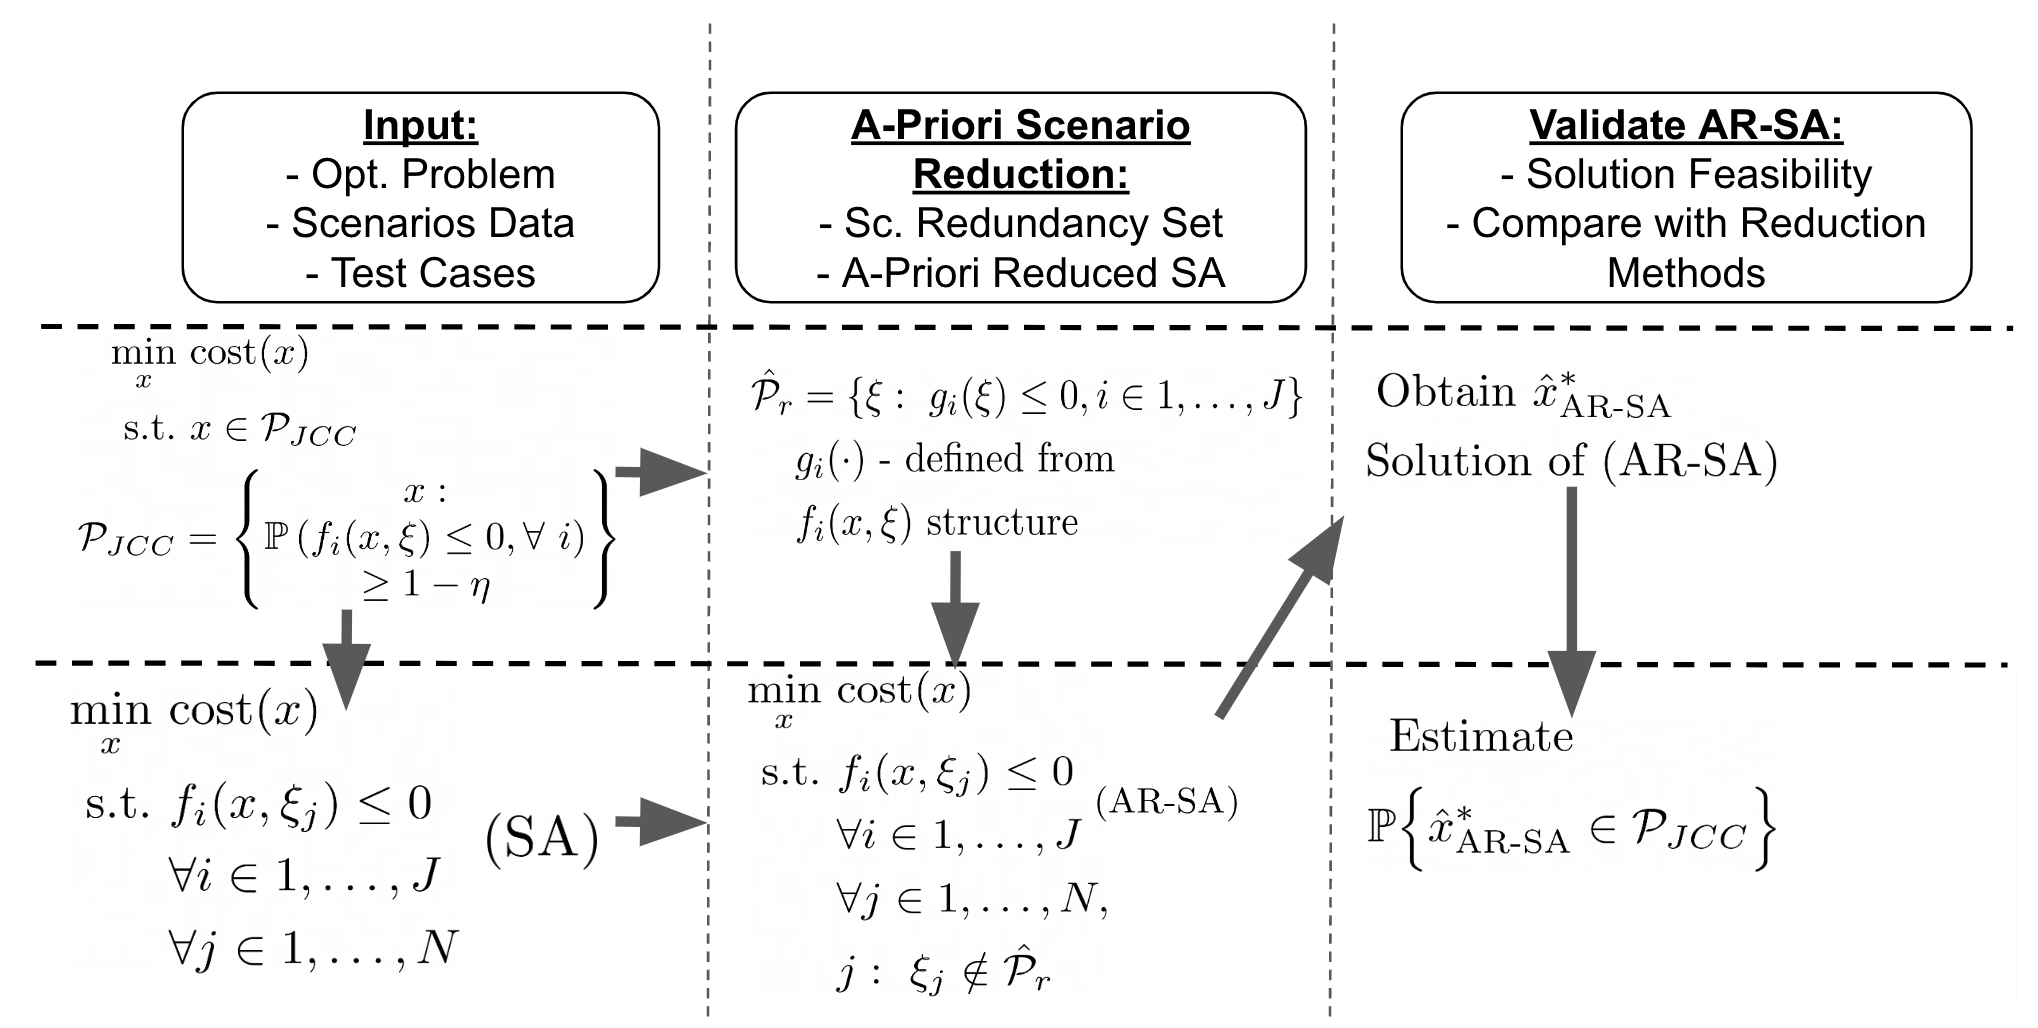
\includegraphics[width=1.\textwidth]{Dissertation/images/dynamic//scheme.png}
    \caption{AR-SA workflow.}
    \label{fig:workflow}
    \vspace{-1mm}
\end{figure}

The rest of this chapter is organized as follows. Section~\ref{sec:setup} provides background and problem setup of the multi-stage high-voltage optimal power flow. Section~\ref{sec:chancecontrol} discusses the setup of the multi-step high-voltage OPF with automated generation control. Section~\ref{sec:chancecontrol} formulates the chance-constrained problem under consideration. Section~\ref{sec:apriori} presents the sketch of the a-priori sample reduction approach, formalizes, and proves its validity. Furthermore, we prove that AR-SA (reduced data-driven approximation) theoretically requires fewer data samples to produce a reliable solution than classical SA. Section~\ref{sec:emp} compares AR-SA with classical Monte Carlo-based SA and other scenario reduction methods such as Fast Forward (FF), Simultaneous Backward (SB), and the clustering K-Means method.

Finally, the conclusion is in Section \ref{sec:conclusion}.
%\vspace{-4mm}
\section{Background and Problem Setup}\label{sec:setup}
\subsection{DC Optimal Power Flow}
%\vspace{-1mm}
The high-voltage DC model is a widely used load flow model in power systems. 

Let $G = (V, E)$ be a power system graph with the set of $n$ nodes (buses) $V$ and the set of $m$ lines (edges) $E$; 
%
$p \in \mathbb{R}^{n_g}$, $p_d \in \mathbb{R}^{n_d}$, and $\theta\in\mathbb{R}^{n}$ be vectors representing power generations, demands, and phase angles, respectively. 

The system is balanced so the sum of all power injections is zero, $\sum_{i \in V} p^i = \sum_{i \in V} p^i_d$.
For clarity we designate one bus as the slack bus, with its phase angle set as $\theta_s = 0$. 
The components of admittance matrix $B$, $B \in \mathbb{R}^{n \times n}$, denoted as $B^{ij}$, are non-zero if there is a line between buses $i$ and $j$. For each node $i$, $B^{ii}$ is defined as the negative sum of the off-diagonal elements $B^{ij}$ with $j \neq i$. 
The DC power flow equations, security and constraints for $i \in V, (i,j)\in E$ are:% expressed as follows:
\vspace{-3mm}
\begin{gather*}
p-p_{d} = B \theta, \!\sum_{i=1}^{n_g} p^i = \!\!\!\sum_{i=1}^{n_d} p^i_d, 
\underline{p}^i_g \leq p^i_g \leq \overline{p}^i, |\theta^i - \theta^j| \leq \bar{\theta}^{ij}
\vspace{-2mm}
\end{gather*}
These equations represent the DC power flow and enforce generation and reliability constraints. 

% \end{comment}
The DC Optimal Power Flow (DC-OPF) feasibility set is linear, determined by voltage phases and power generation within grid topology, line characteristics (admittance matrix), and power demand \cite{wood2013power} (Chapter 4.1.4). The objective is to find an economically optimal active power generation profile across available generators while adhering to technical limits and system demand, which define rules and technical limits on power transfer throughout the system.
The feasibility set of DC-OPF can be reformulated as a polytope $P = {p: Wp \leq b}$ in the vector space of active power generations $p \in \mathbb{R}^{n_g}$, where $W \in \mathbb{R}^{J \times n_g}$ and $b \in \mathbb{R}^J$. Here, $n_g$ denotes the number of controllable generators, and $J$ represents the number of constraints \cite{lukashevich2021importance}, \cite{ lukashevich2021power, owen2019importance}. Reliability constraints are violated when the power generation vector $p$ falls outside the polytope $P$.

Solving DC-OPF consists of finding the power flow by minimizing a convex cost of power generation $c(p_g)$ subject to the constraints defined by $P$. 
\vspace{-1mm}
\subsection{Source of uncertainty and AGC}
\label{sec:fluctuations}
\vspace{-2mm}

The fluctuations affect the power balance in the system and are typically managed through primary and secondary control \cite{machowski2020power}. In this chapter, we consider linear Automatic Generation Control (AGC). The AGC recourse adjusts the generation to a new setpoint $p^{t+1} = p^t + \alpha \xi^t$ \cite{roald2017chance,baros2021examining,mezghani2020stochastic} with $p^t \in \mathbb{R}^{n_g}$, $\alpha \in \mathbb{R}^{n_g}$, and $\xi^t \in \mathbb{R}$ representing the \emph{total} demand-generation imbalance.

The participation factors $\alpha$ for secondary control can slightly vary, enabling long-term grid stability and fast control~\cite{machowski2020power}. 


The total system imbalance $\xi^{t}$ is a sum of power fluctuations caused by an intermittency of renewable generation, demand instability, and intra-day electricity trading. More specifically, if a power system has nodes $\mathcal{B}$, $\xi^t = \sum_{b \in \mathcal{B}} (\xi_b^d)^t - (\xi_b^g)^t$, where $(\xi_b^d)^t$ and $(\xi_b^g)^t$ are random variables that model fluctuations at bus $b$, at time stamp $t$ in demand and generation, respectively. Depending on the source, these random variables follow various distributions. For example, if a bus $b$ contains a PV generator, then $(\xi_b^g)^t$ follows beta distribution \cite{wang2010probabilistic}, if there is a wind farm, wind speed distribution is Weibull, however, power output can be vary from turbine to turbine \cite{dhople2012framework}. Nevertheless, $\xi^t$ is a sum of random variables and, due to the Lyapunov or Lindeberg-Feller Central Limit Theorem \cite{scholz2011central}, follows Gaussian distribution \cite{rouaud2013probability, draper2021practical}. We also checked the validity of this assumption by applying Shapiro-Wilk normality test \cite{shapiro1965analysis} on time series of load-renewable generation imbalance estimated from RTS-GLMC data \cite{barrows2019ieee}. The latter project incorporates time series for demand, hydro, rooftop PV, PV, wind farms generations. The Shapiro-Wilk testing revealed that, on significance level of $\alpha=0.05$, the $H_0$ hypothesis (the generation-demand imbalance is distributed normally) is rejected only for August and November. The testing results are monthly-wise and presented in Table \ref{tab:shapiro-wilk}. Thus, the assumption that $\xi^t$ is Gaussian is valid. We further consider stacked temporal uncertainty vector $\xi = (\xi^1, \dots, \xi^T) \sim \mathcal{\mu, \Sigma}$ and $\Sigma$ here models temporal correlations.

Given the samples $X_1, \dots, X_{n_s}$, the Shapiro-Wilk test uses the following $H_0$ hypothesis: the samples are drawn from a normal distribution $\mathcal{N}(\mu_s, \sigma^2_s)$. The alternative $H_1$ is that the population is not normal. This test is one-tailed. The following statistic is applied: $W_{\textup{S-W}} = \frac{\left( \sum_{i=1}^{n_s} a_i X_{(i)} \right)^2}{\sum_{i=1}^{n_s} \left( X_i - \bar{X}\right)^2}$, where $\bar{X} = \frac{1}{n_s} \sum_{i=1}^{n_s} X_i$ and $X_{(i)}$ -- $i^{\textup{th}}$ order statistic. The coefficients $a_i$ are defined using samples $Z_1, \dots Z_{n_s} \sim \mathcal{N}(0, 1)$. Denote $V$ as the covariance matrix of the standard normal samples: $V_{ij} = \mathbb{E}\left[ (Z_{(i)} - m_i)(Z_{(j)} - m_j) \right]$, where $m = (m_1, \dots, m_{n_s})^\top$ is the vector of expected values of order statistics of $Z_{(1)}, \dots, Z_{(n_s)}$. Finally, $(a_1, \dots, a_{n_s})^\top = \frac{m^\top V^{-1}}{C}$ with $C = \left( m^\top V^{-1} V^{-1} m \right)^{1/2}$. Essentially, $W_{S-W}$ statistic is a relation between two empirical estimates of the $\sigma^2_s$. Thus, if the samples $X_1, \dots, X_{n_s}$ are drawn from normal distribution, $W$ is close to its maximum value of $1$, otherwise, it tends to its minimal value of $n_s a_1^2 / (n_s - 1)$ which is close to $0$ in practice \cite{shapiro1965analysis}.

\begin{table}[t]
\caption{$p$-values and Shapiro-Wilks (SW) Gaussianity test results on RTS-GLMC data. 
    }
    \centering
        \begin{tabular}{|c|c|c|}
        \toprule
        Month & $p$-value & SW decision $\alpha=0.05$ \\
\midrule
January & 0.108 & Looks like Gaussian (fail to reject $H_0$) \\
February & 0.167 & Looks like Gaussian (fail to reject $H_0$) \\
March & 0.429 & Looks like Gaussian (fail to reject $H_0$) \\
April & 0.178 & Looks like Gaussian (fail to reject $H_0$) \\
May & 0.140 & Looks like Gaussian (fail to reject $H_0$) \\
June & 0.162 & Looks like Gaussian (fail to reject $H_0$) \\
July & 0.334 & Looks like Gaussian (fail to reject $H_0$) \\
August & 0.000 & Does not looks like Gaussian (reject $H_0$) \\
September & 0.056 & Looks like Gaussian (fail to reject $H_0$) \\
October & 0.562 & Looks like Gaussian (fail to reject $H_0$) \\
November & 0.023 & Does not looks like Gaussian (reject $H_0$) \\
December & 0.173 & Looks like Gaussian (fail to reject $H_0$) \\
\bottomrule
        \end{tabular}
    % }
    \label{tab:shapiro-wilk}
\end{table}

Below we assume that the fluctuations are Gaussian with the mean and covariance recoverable from historical data~\cite{roald2017chance, owen2019importance}.
We consider the system evolution driven by fluctuations and formulate an optimization problem to obtain an economically optimal control strategy and initial system setpoint that satisfy JCC on technical limits and demand.

Table~\ref{tab:notation} summarizes the chapter's notation. We use upper indices for elements of vectors and matrices, lower-case letters for probability density functions (PDFs), and upper-case letters for cumulative distribution functions (CDFs). When it does not lead to confusion, we use $\mathbb{P}$, $\mathbb{E}$, $\mathbb{V}$ to denote probability, expectation, and variance without mentioning a distribution. 
%\vspace{-3mm}

\begin{table}[t]
    \centering
    \caption{Chapter notation.}
    \begin{tabularx}{\textwidth}{|m{1cm}|X|m{1.6cm}|X|}
        \toprule 
        ${P}$ & DC-OPF feas. set & $P_{JCC}$ & JCC DC-OPF feas. set \\
        $p$ & vector of generation & $n_g$ & \# of controllable gen. \\
        $\alpha$ & participation factors & $J$ & \# of constraints in $P$ \\
        $T$ & \# of modeling timestamps & $\mathcal{N}(\mu, \Sigma)$ & Gaussian distribution \\  
        $\xi^t$  & power balance mismatch at timestamp $t$ & $\Phi$ & CDF of standard Gaussian r.v. \\
        $I$ & identity matrix & $R$ & rampup/down limits \\
        $\mathcal{P}_r$ & theoretical redundancy set & $\hat{\mathcal{P}}_r$ & sufficient redundancy set\\
        \bottomrule
    \end{tabularx}
    \label{tab:notation}
    %\vspace{-4mm}
\end{table}
\section{Optimal multi-stage control under uncertainty}\label{sec:prob}
In this section, we formulate the multistage chance-constrained DC-OPF. We begin by describing the uncertainty in the system and the impact on control and optimization. Next, we address the Automated Generation Control (AGC). Further, we present the complete chance-constrained optimization problem. Accordingly, we introduce the Scenario Approximation (SA) of the chance constrainted control proposed. Finally, we address and define the redundant scenarios for this problem and present a procedure to efficiently sample them. 
\vspace{-3mm}
The power mismatch at timestamp $t=1, \dots, T$ is given by:
\begin{gather}\label{eq:power-balance}
{\bold 1}^\top p^t - {\bold 1}^\top p_d - \xi^t = {\bold 1}^\top p^{t-1} - {\bold 1}^\top p_d + \xi^t - \xi^t = 0.
\end{gather}
i.e., this control strategy keeps the system balanced. Notice that $\xi^t$ represents the overall fluctuation, including load and generation uncertainties, and $p_d$ remains constant in time.
% \vspace{-4mm}
\section{Chance constraint multi-stage control}
\label{sec:chancecontrol}
In this section, we introduce the JCC discrete-time dynamic DC-OPF with AGC, reformulate it compactly, and outline a data-driven approximation leading to a solution feasible for the original chance-constrained problem with high probability.
%\vspace{-4mm}
\subsection{Chance constrained optimization}
\vspace{-1mm}

Consider a dynamical system with $T$, $T<\infty$, timestamps, and $\xi^t$, $1 \le t\le T$ - total power mismatch due to uncertainties at timestamp $t$. 
Let individual uncertainties follow a Gaussian distribution: $\xi^t \sim \mathcal{N}(0, (\sigma^t)^2)$, $1\le t\le T$, so that $\xi \sim \mathcal{N}(0, \Sigma), ~\Sigma \in \mathbb{R}^{T\times T}$ with marginals distributed as $\mathcal{N}(0, (\sigma^t)^2)$. The temporal binding between system timestamps is modeled through the ramp rates of generators, ensuring realistic rates of change in power outputs as $|p^t_i - p^{t-1}_i| \leq R_i$, where $R_i > 0$. The discrete-time dynamic chance-constrained optimization problem is then: 
\vspace{-3mm}
\begin{align}
        & \hspace{32mm} \min_{p^t, \alpha} \mathbb{E} \sum_{t=1}^T c(p^t) \label{eq:optimal_control}, \qquad \texttt{s.t.:} 
        \\ 
        & \; \mathbb{P} 
        \begin{pmatrix}
                Wp^t \leq b, p^t = p^{t-1} + \alpha\xi^t, |p_k^t - p_k^{t-1}| \leq R_k,\\
                 1 \leq k \leq n_g, ~1\leq t \leq T
        \end{pmatrix} \geq 1 - \eta.\nonumber
\end{align}
where $\eta\in (0, 1/2]$, $\mathbb{P}$ is a joint measure induced by the uncertainty distribution, and $\alpha \in \mathbb{R}^{n_g}$ is participation factors. 
%$\sum_{i=1}^{n} \alpha_i = 1, ~ \alpha_i \geq 0$ and $\alpha_i$ on loads is equal to zero. 
%\begin{equation}
%    \begin{aligned}
%        \min_{p_t} &~\mathbb{E} \sum_{t=1}^T c(p^t) \\
%\texttt{s.t. }  \mathbb{P} &
%                \begin{pmatrix}
%                Wp_t \leq b \\
%                 p_t = p_{t-1} + \alpha \sum_{k} \xi_{t, k} \\
%                 \sum_{i=1}^{n_g} \alpha_i = 1, ~ \alpha_i \geq 0 \\
%                 |\alpha_i \sum_{k}\xi_{k,t}| \leq (\Delta_{p})_i
%                \end{pmatrix} \geq 1 - \eta
%    \end{aligned}
%    \label{eq:optimal_control}
%\end{equation}

%{\color{blue} I am not sure on the equation above in its initial form. TBD} {\color{red} Please see my comment with href on Deep's chapter}
%
%{\color{blue} stopped here}

%First, one should note that $\sum_{k} \xi_{t, k} \sim \mathcal{N}(0, \sum_{k} \sigma^2_{i,k})$. This implies that $p_t \sim{N}(p_0, \sum_{\tau=1}^t \sum_{k} \sigma^2_{\tau,k})$. Which makes the $\mathbb{E}c^\top p_t = c^\top p_0$. The latter mean that the average generation cost depends only on the initial generation set-point.

%Secondly, one may deduce from AGC rule that $p_t = p_0 + \sum_{\tau=1}^t \sum_{k} \xi_{\tau,k}) = p_0 + \xi_t$, where $\xi_t \sim \mathcal{N}(0, \sum_{\tau=1}^t \sum_{k} \sigma^2_{\tau,k}))$. For simplicity, we denote $\sigma^2_t = \sum_{\tau=1}^t \sum_{k} \sigma^2_{\tau,k}$.

%Thus, simplifying, one can reformulate Problem %\ref{eq:optimal_control} as follows:
%\begin{equation}
%    \begin{aligned}
%        \min_{p_t} &~c^\top p_0 \\
%\texttt{s.t. }  \mathbb{P} &
%                \begin{pmatrix}
%                Wp_t \leq b \\
%                 p_t = p_{0} + \xi^t \\
%                 \sum_{i=1}^{n_g} \alpha_i = 1, ~ \alpha_i \geq 0 \\
%                 |\alpha_i \xi_{t}| \leq (\Delta_{p})_i
%                \end{pmatrix} \geq 1 - \eta
%    \end{aligned}
%    \label{eq:optimal_control_1}
%\end{equation}
% An equivalent formulation to the problem above is
% \[\min_{p^t, \alpha} \mathbb{E} \sum_{t=1}^T c(p^t) \]
% \begin{equation}
%     \begin{aligned}
%         & \texttt{subject to:}  
%         \\ 
%         & \; \mathbb{P} 
%         \begin{pmatrix}
%                 Wp_0 + W \alpha\sum_{t\le \tau} (\xi^t)\leq b, 0 \le \tau\le T \\
%                 %p^t = p^{t-1} + \xi^t + D(\alpha) \delta p^t,  1\le t\le T \\
%                 |\alpha_k \xi^\tau| \leq R_k, \le 1\le k\le n_g , 0\leq \tau \leq T
%         \end{pmatrix} \geq 1 - \eta.
%     \end{aligned}
%     \label{eq:optimal_control_2_pre} 
% \end{equation}
% where for $t = 0$ we assume no uncertainty, i.e, $\xi^0 = 0$. 
A compact statement of the Problem \eqref{eq:optimal_control} is:
%assuming no uncertainty for $t = 0$:
\vspace{-3mm}
\[\min_{p^t, \alpha} \mathbb{E} \sum_{t=1}^T c(p^t) \]
\vspace{-3mm}
\begin{equation}
    \begin{aligned}
        \!\!\texttt{s.t.:}  & \mathbb{P}\!\! 
        \begin{pmatrix}
                \mathcal{W}^p p^0 + E^\tau \mathcal{W}^{\alpha} \cdot \alpha \leq \beta, 0 \leq \tau \leq T 
        \end{pmatrix}\!\geq\!1 - \eta,\!\!\!
    \end{aligned}
    \label{eq:optimal_control_2} 
\end{equation}

% \begin{subequations}\label{eq:optimal_control_2} 
%     \begin{alignat}{1}
%         & \texttt{subject to:}  
%         \\ 
%       & \; \mathbb{P} 
%         \begin{pmatrix}
%                 \mathcal{W}^p p^0 + E^\tau \mathcal{W}^{\alpha} \cdot \alpha \leq \beta, 0 \leq \tau \leq T 
%         \end{pmatrix} \geq 1 - \eta.\label{subeq:JCC} \\
%     \end{alignat}
%   \end{subequations}
where $E^\tau \in \mathbb{R}^{J+2n_g \times J + 2n_g}$ is a diagonal matrix with first $J$ diagonal elements equal $(1^\tau) ^\top \xi$, the rest are $(e^\tau)^\top\xi$. Here
%of $J$ vectors $1^{\tau}$ followed by $2 \times n_g$ vectors $e^\tau$, where  
$1^{\tau} \in \mathbb{R}^T$ has components $1^{\tau}_i = 1, ~ 0 \leq i \leq \tau, ~ 0$ otherwise. The vector $e^\tau_i = 1, ~ i=\tau, e^\tau_i = 0$ in the other case. Later in the chapter, given specific $i:1 \leq i \leq J + 2n_g$ and $1\leq \tau \leq T$ we refer the second term components as $(E^\tau_i)^\top\xi \cdot (\omega_i^\alpha)^\top \alpha$, where $E^\tau_i$ is $1^\tau$ for $i \leq J$ and $e^\tau$ for $i > J$.
Matrices are obtained as vertical stacks: $\mathcal{W}^p = \left( W^\top, 0, 0 \right)^\top$ and $\mathcal{W}^\alpha = \left(W^\top, I_{n_g}, -I_{n_g} \right)^\top$, $\mathcal{W}^p, ~ \mathcal{W}^\alpha \in \mathbb{R}^{(J + 2 \cdot n_g)\times n_g}$. The right hand side of Eq.~\eqref{eq:optimal_control_2}, $\beta = \left(b^\top, R, R \right)^\top$ with $R = \{R_k\}_{k=1}^{n_g}$ being the vector of ramp up/down limits. %Essentially, the compact formulation includes grid constraints together with ramp up/down limits. 
We use subscript to refer to rows of the matrices $\mathcal{W}^p, \mathcal{W}^\alpha, E^\tau$; $\omega_i^{p}, ~ \omega_i^{\alpha}$ for the rows of matrices $\mathcal{W}^p, \mathcal{W}^\alpha$. %{\color{red} Could you please proof read the above for clarity?} %{\color{blue} Finally, we introduce short notation for JCC from \eqref{eq:optimal_control_2}: $\pi(p^0, \alpha) = \mathbb{P} \left(\mathcal{W}^p p^0 + E^\tau \mathcal{W}^{\alpha} \cdot \alpha \leq \beta, 0 \leq \tau \leq T \right)$.}
%Note that $\xi^\top e^{\tau} \sim \mathcal{N}(0, \sum_{t=1}^\tau (\sigma^t)^2)$ for $\tau >0$, otherwise it equals $0$.
%Notice, that all constraints in Prob.~\eqref{eq:optimal_control} are linear that allows to equally setup~Prob.~\eqref{eq:optimal_control_2} as follows:
%\begin{align}
%& \qquad \min_{p_t} \mathbb{E} \sum_{t=1}^T c(p^t) \label{eq:reduced-form}\\ 
%        & \texttt{subject to:}  \; \mathbb{P} \left({\cal W} \xi \le \beta \right) \le 1-\eta, \nonumber 
%\end{align}
%where $\beta$ linearly depends on $p_0$ and $b$, and $\xi = (\xi^1; \dots; \xi^T)$ is $nT\times 1$ vector. 
%
%
%
%One should note that the constraints that are defining safe operating regime and AGC recourses are as follows: $W(p_0 + \alpha \xi_t) \leq b$.
%
%One can further reformulate the polytope under probability, obatining the following compact form: $\mathcal{P} = \{ \mathcal{W}^p p + \mathcal{W}^{\alpha}\alpha \circ \Pi_T \vec{\xi} \leq \beta\}$.
%Here $\circ$ is Hamadard's product, $\mathcal{W}^p = [W^\top, \dots, W^\top, \mathcal{0}_{3 n_g \times n_g}]^\top$, $\mathcal{W}^{\alpha} = [(WC^{\alpha})^\top, \dots, (C^{\alpha})^\top, C^{\alpha}, -C^{\alpha}, -C^{\alpha}]^\top$, $\beta = [b^\top, \dots, b^\top, \Delta_p, \Delta_p, \mathcal{0}_{n_g}]^\top$,
%i.e., constraint matrices and right hand side are duplicated $T$ times and stacked with ramp-up and ramp-down limits, and, finally, inequalities that impose $\alpha \in S^1_{\Delta}$. 
%Also, $C^{\alpha}$ is defined to eliminate $\sum_{\alpha} = 1$ constraint: for $i\neq 1, ~j \neq 1$ $C^{\alpha}_{ii}=1, ~ C^{\alpha}_{ij}=1, ~ C^{\alpha}_{1i} = -1$. 
%Random vector $\vec{\xi} \sim \mathcal{N}(\vec{0}, \texttt{diag}(\sigma_1^2, \dots, \sigma^2_T))$ and matrix $\Pi = [\Pi_T^\top \mathbb{0}_{n_g \times T}]^\top$, where $\Pi_T \in \mathbb{R}^{T \cdot m ~\times~ T}, ~ (\Pi_T)_{ij} = 1$ if $k \cdot T\leq j \leq (k+1) \cdot (T)$ and $i = k, ~ k = 0, \dots, T$, otherwise, it is $0$.
%This matrix allow to get a component of $\vec{\xi}$, corresponding to a snapshot $\tau \in 1, \dots, T$ and zeros for the constraints that does not include any stochasticity, namely, $\alpha_i \geq 0, ~ i=1, \dots, n_g$. Let us denote $J$ as the length of $\beta$, which means the total number of inequality constraints that define the deterministic feasibility polytope.
%
%Thus, the problem can be compactly rewritten as 
%
%\begin{equation}
%    \begin{aligned}
%        \min_{p_t} &~c^\top p_0 \\
%\texttt{s.t. }  \mathbb{P} &
%                \begin{pmatrix}
%                \mathcal{W}^p p_0 + %\mathcal{W}^{\alpha} \circ \Pi \vec{\xi} \leq \beta
%                \end{pmatrix} \geq 1 - \eta
%    \end{aligned}
%    \label{eq:optimal_control_compact}
%\end{equation}
%
%Further, we refer to the feasibility set of the Problem \ref{eq:optimal_control_2} as~$\mathcal{F}$.

% Eliminating $\delta p^t$ leads to
% \begin{equation}
%     \begin{aligned}
%         & \qquad \min_{p_t} \mathbb{E} \sum_{t=1}^T c(p^t) \\
%         & \texttt{subject to:}  
%         \\ 
%         & \; \mathbb{P} 
%         \begin{pmatrix}
%                 p_0 + W \sum_{t\le \tau}( I - D(\alpha)) \delta p^t\leq b, t\le \tau \\
%                 %p^t = p^{t-1} + \xi^t + D(\alpha) \delta p^t,  1\le t\le T \\
%                 |\xi_k^t + \alpha_k\delta p^t| \leq \Delta_k, \le 1\le k\le n \\
%                 \delta p^t = - \sum_{i\le n}\xi^t_i, 1\le t \le T %\textup{\color{red} it should be a scalar}
%         \end{pmatrix} \geq 1 - \eta.
%     \end{aligned}
%     \label{eq:optimal_control_2} 
% \end{equation}
%\vspace{-5mm}
\subsection{Scenario approximation of chance constrained control}
A Scenario Approximation (SA) of the Problem~\eqref{eq:optimal_control_2} via the set of scenarios $\xi(j), ~ j=1,\dots, N$, implying a separate set of constraints for each one, is%i.e., constraints under probability are repeated for each sampled scenario $\xi(j)$
:
\vspace{-3mm}
    \begin{align}
        & \qquad \min_{p^0, \alpha} c(p^0), \qquad \texttt{s.t.:}  \label{eq:optimal_control_sampling_02} 
        \\ 
         \forall j, 1\leq j \leq N\!\!:& \;  \mathcal{W}^p p^0 +  (E^\tau)^\top \xi(j) \mathcal{W}^{\alpha} \alpha \leq \beta, 0 \leq \tau \leq T.\nonumber
        %\end{pmatrix} \geq 1 - \eta.
\end{align}

which is built on scenarios, or data samples, $\xi(j)$, $1\le j \le N$ incapsulated in matrices $E^\tau(j)$. %Further, we denote $\zeta^\tau = \sum_{t < \tau} \xi^t$ which distributed as $\mathcal{N}(0, (\tilde{\sigma}^\tau)^2)$ with  $(\tilde{\sigma}^\tau)^2 = \sum_{t < \tau} (\sigma^t)^2$.
% Additionally, we rewrite the problem above in a more compact way by combining all of the inequality constraints into one matrix inequality:
% \begin{equation}
%     \begin{aligned}
%         & \qquad \min_{p_t} \sum_{j=1}^N\sum_{t=1}^T c(p^t) \\
%         & \hspace{-4mm}\texttt{subject to:}  
%         \\ 
%         & \;  \mathcal{W}_T\left(p_0 +  \alpha\sum\limits_{t\le \tau} \xi^t(j) \right)\leq \beta_T, t=0\le T,
%         %\end{pmatrix} \geq 1 - \eta.
%     \end{aligned}
%     \label{eq:optimal_control_sampling_02} 
% \end{equation}
% here we assume that for $t=0$ $\xi^0 = 0$. The matrix $\mathcal{W}_T$ and the right hand side $\beta_T$ are simply describe
%{\color{blue}Sasha, check the equation above} {\color{red}im not sure about this deltap... it should be dependent on $(j)$ as well, as i see}
\vspace{-2mm}
% SA offers practical benefits but demands a huge number of samples to obtain a reliable solution \cite{calafiore2006scenario}. Reduction strategies, particularly a-priori methods, are underexplored {\color{blue} for JCC problems in power systems}. By reducing data samples, the number of constraints in the approximation decrease, enhancing optimization tractability. Ensuring approximation reliability, we analyze a-priori data sample redundancy conditions and provide reliability guarantees for the solution of the resulting data-driven approximation.
Scenario approximation is very attractive from the practical perspective but requires an extreme number of samples to achieve reasonable accuracy \cite{calafiore2006scenario}. The reduction of the amount of samples in data-driven approximations is poorly studied area, especially, a-priori strategies. Data samples usage reduction reduces the number of constraints in the SA, making the underlying optimization problem more tractable. However, it is important to guarantee that the approximation reduction does not lead to a corruption of the approximate solution. To this end, we analyse a-priori data sample redundancy for the problem under study and prove approximate solution reliability guarantees.
%
The importance sampling approach we leverage in this chapter consists of two steps. First, we derive a conservative outer approximation to the set of optimal solutions of Problem~\eqref{eq:optimal_control_2}. Based on this, we add a sequence of deterministic constraints, allowing us to eliminate redundant scenarios from the scenario approximation. Finally, instead of using vanilla Monte-Carlo, we sample from a proxy distribution (importance distribution) has significantly less redundant scenarios. %This approach improves the sample complexity bound and enhances solution reliability \cite{lukashevich2021importance}.
%
%
% Finally, the importance sampling chance constrained problem extension is: 
% \begin{equation}
%     \begin{aligned}
%         & \qquad \min_{p_t} \sum_{j=1}^N\sum_{t=1}^T c(p^t) \\
%         & \hspace{-4mm}\texttt{subject to:}  
%         \\ 
%         & \;  p_0 + W\alpha \sum\limits_{t\le \tau} \xi^t(j)\leq b, t\le \tau \\
%                 %p^t = p^{t-1} + \xi^t + D(\alpha) \delta p^t,  1\le t\le T \\
%               &  |\alpha_k \xi^t(j)| \leq \Delta_k, \le 1\le k\le n\\
%               & p = (p^1, \dots, p^T) \in C
%         %\end{pmatrix} \geq 1 - \eta.
%     \end{aligned}
%     \label{eq:optimal_control_sampling-2} 
% \end{equation}
% where scenarios $\xi^t_k(j) \sim D$, $1\le j \le N$, and $C$ is the above mentioned outer approximation of the optimal solutions set.
%\vspace{-4mm}
\section{A-priori scenario redundancy}
\label{sec:apriori}
We introduce the concept of redundant data samples within a SA by defining analytical conditions for data redundancy in a JCC multi-timestamp DC-OPF. We also provide the minimum number of scenarios required to achieve a $1 - \rho$ reliable solution, i.e., a solution feasible for Problem \eqref{eq:optimal_control_2} with a probability of $1 - \rho$, and derive reduction factors based on the measure of the analytical redundancy set. %.{\color{red} sounds confusing.. Which one is that?}
%\vspace{-4mm}
\subsection{Redundant scenarios}
%\vspace{-1mm}
In this subsection we present an approach and theorems that are aiming for a-priori scenario redundancy classification. First, we begin with formalization of data sample redundancy and its illustration. Next, we move to formal statements that define an inner approximation of the redundancy set $\mathcal{P}_r$ that classify data samples whether they are redundant. 

\begin{definition}
\label{def:redundant}
% Consider SA \eqref{eq:optimal_control_sampling_02} that has a solution $(\hat{p}^0_{\mathcal{I}}, \hat{\alpha}_{\mathcal{I}})$ which is feasible for the JCC problem \eqref{eq:optimal_control_2} and a set of scenarios~$\mathcal{I}$. An set of scenarios ${\cal I}_r$ is redundant iff it does not change the solution, $(\hat{p}^0_{\mathcal{I}}, \hat{\alpha}_{\mathcal{I}}) = (\hat{p}^0_{\mathcal{I} \setminus \mathcal{I}_r}, \hat{\alpha}_{\mathcal{I} \setminus \mathcal{I}_r})$.
Let $\mathcal{I} = \{1, \dots, N\}$. Scenarios indexed with $\mathcal{I}_r \subset \mathcal{I}$ are called redundant iff a solution of SA with constraints corresponding to scenarios indexed with $\mathcal{I}_r$ are omitted - $(\hat{p}^0_{\mathcal{I} \setminus \mathcal{I}_r}, \hat{\alpha}_{\mathcal{I} \setminus \mathcal{I}_r})$ - is feasible for initial JCC \eqref{eq:optimal_control_2} and solution of SA $(\hat{p}^0_{\mathcal{I}_r}, \hat{\alpha}_{\mathcal{I}_r})$ with constraints corresponding to those scenarios indexed with $\mathcal{I}_r$ is not feasible for JCC \eqref{eq:optimal_control_2}.
\end{definition}

%{\color{red} the definition is confusing (english), could not we tell in words that ``A subset of scenarious $I' \in I$ is redudant, iff the solutions of Problem (3) with scenarious $I$ and $I\setminus I'$ are the same''?}
The redundancy concept is illustrated in Figure~\ref{fig:idea}. All data samples can be divided into redundant and non-redundant, depending on whether they are inside or outside the set $\mathcal{P}_r$ with an unknown structure. In practice, one can derive inner approximations $\hat{\mathcal{P}}_r$ of $\mathcal{P}_r$. The latter can be used to classify data by redundancy in SA. Our goal is to define conditions for a-priori identification of redundant scenarios. Consider a set $\mathcal{P}_r$ containing all redundant samples (scenarios indexed by $\mathcal{I}_{r}$ from Def.~\ref{def:redundant}). Keeping only these samples from $\mathcal{P}_r$ results in an infeasible solution for Problem \eqref{eq:optimal_control_2}. But keeping scenarios outside of $\mathcal{P}_r$ yields a feasible solution. Since it's challenging to analytically define $\mathcal{P}_r$, we aim to construct an inner approximation $\hat{\mathcal{P}}_r$. Such approximation provides a sufficient condition for identifying redundant samples. We derive the inner redundancy set $\hat{\mathcal{P}}_r$ for efficient scenario generation. Additionally, we employ a standard technical assumption \cite{campi2011sampling},  that ensures that problems with finitely many constraints are feasible% and non-binding from the practical standpoint
:
\begin{assumption}\label{asmp:10}
For all possible uncertainty realizations $\xi(1), \dots, \xi(N)$, optimization problem \eqref{eq:optimal_control_sampling_02} is either infeasible or has a unique optimal solution.
\end{assumption}
We provide an example that addresses the redundancy concept in Figure \ref{fig:idea} we present a simplified illustration of the concept. Our aim is to define conditions that give a-priori knowledge on the redundancy of a given data sample. Assume that unknown set $\mathcal{P}_r$ contains all redundant samples, i.e., scenarios indexed by $\mathcal{I}_{r}$ from Definiton \ref{def:redundant}. Notice that keeping only those samples from $\mathcal{P}_r$ would lead to a solution of the approximation that will be out of $P_{JCC}$, i.e., infeasible for Problem \eqref{eq:optimal_control_2}. On the other hand, keeping only those scenario that are outside of $\mathcal{P}_r$, i.e., indexed by $\mathcal{I} \setminus \mathcal{I}_r$, would lead to a feasible solution for Problem \eqref{eq:optimal_control_2}. In general it is not possible to analytically define $\mathcal{P}_r$, thus, we aim to construct an inner approximations for $\mathcal{P}_r$, namely, $\hat{\mathcal{P}}_r$. In other words, analytical definitions of $\hat{\mathcal{P}}_r$ allow one to obtain sufficient conditions on data sample redundancy based on its belonging to this set. We derive the inner redundancy set $\hat{\mathcal{P}}_r$ for proxy distribution that allows for efficient scenario generation. 
% \begin{assumption}\label{asmp:10}
% Assume that for all possible uncertainty realizations $\xi(1), \dots, \xi(N)$, the optimization problem \eqref{eq:optimal_control_sampling_02} is either infeasible or, if feasible, it attains a unique optimal solution.
% \end{assumption}
\def\shift{2.7}
\def\shiftt{2.}
\def\shiftuselesssample{0.3}
\def\shiftusefulsample{1.1}
\def\xx2{0 + \shiftt}
\def\yx2{0 - \shiftt}
\def\threshold{33} 
\tikzset{snake it/.style={decorate, decoration={coil,amplitude=1pt, segment length=9pt}}}
\begin{figure}
\begin{minipage}{0.35\linewidth}
    \centering
        \begin{tikzpicture}[scale=0.7, node distance={15mm}, thick, main/.style = {draw, scale=.5}] 
        \clip (0,2) rectangle + (6,-7);
        
        \coordinate (x2) at (\xx2, \yx2);
        \coordinate (x2origin) at (\xx2 + 1.5, \yx2 - 2);
        \draw[olive] (x2) circle (1pt);
        \draw (x2) ++(1.5, -2.3) node[olive, above right] (tmp) {$(\hat{p}_{\mathcal{I}}, \hat{\alpha}_{\mathcal{I}})$};
        \draw[->, olive] (x2origin) -- (x2);
        %Deterministic set - outer guy
        \coordinate (a) at ( 4.755282581475767 , 1.545084971874737 );
        \coordinate (b) at ( 3.061616997868383e-16 , 5.0 );
        \coordinate (c) at ( -4.755282581475767 , 1.5450849718747375 );
        \coordinate (d) at ( -2.9389262614623664 , -4.045084971874736 );
        \coordinate (e) at ( 2.9389262614623646 , -4.045084971874738 );
        %linking outer guy
        \draw (a) -- (b);
        \draw (b) -- (c);
        \draw (c) -- (d);
        \draw (d) -- (e);
        \draw (e) -- (a);
        %annotating outer guy
        \draw
        (a) ++(0.1, -1.21) node[below] (tmp) {$P$};
        %(tmp.west) -- (PO);
        
        %JCC feasibility set - green guy
        \coordinate (ag) at ( 3.804226065180614 , 1.2360679774997896 );
        \coordinate (bg) at ( 2.4492935982947064e-16 , 4.0 );
        \coordinate (cg) at ( -3.804226065180614 , 1.23606797749979 );
        \coordinate (dg) at ( -2.351141009169893 , -3.2360679774997894 );
        \coordinate (eg) at ( 2.3511410091698917 , -3.2360679774997902 );
        %linking green guy
        \draw [black, snake it] (ag) -- (bg);
        \draw [black, snake it] (bg) -- (cg);
        \draw [black, snake it] (cg) -- (dg);
        \draw [black, snake it] (dg) -- (eg);
        \draw [black, snake it] (eg) -- (ag);
        %annotating green guy
        \draw
        (ag) ++(0., -0.6) node[left, black] (tmp) {${P}_{\textup{JCC}}$};
        %(tmp.west) -- (PO);
        
        %Redundant samples botder - teal
        \coordinate (ar2) at ( 0.9510565162951535 + \shiftt , 0.3090169943749474 - \shiftt);
        \coordinate (br2) at ( 6.123233995736766e-17 + \shiftt , 1.0  - \shiftt);
        \coordinate (cr2) at ( -0.9510565162951535  + \shiftt, 0.3090169943749475  - \shiftt);
        \coordinate (dr2) at ( -0.5877852522924732 + \shiftt, -0.8090169943749473 - \shiftt);
        \coordinate (er2) at ( 0.5877852522924729 + \shiftt, -0.8090169943749476  - \shiftt);
        %linking teal
        \draw [teal, snake it] (ar2) -- (br2);
        \draw [teal, snake it] (br2) -- (cr2);
        \draw [teal, snake it] (cr2) -- (dr2);
        \draw [teal, snake it] (dr2) -- (er2);
        \draw [teal, snake it] (er2) -- (ar2);
        %annotating teal guy
        \draw
        (br2) ++(1em, .1em) node[above, teal] (tmp) {$\mathcal{P}_{r}$};
        %(tmp.west) -- (PO);

        %Inner redundant - purple
        \coordinate (anvc) at ( 0.9510565162951535 * 0.7 + \shiftt , 0.3090169943749474 * 0.7 - \shiftt);
        \coordinate (bnvc) at ( 6.123233995736766e-17 + \shiftt , 1.0 * 0.7  - \shiftt);
        \coordinate (cnvc) at ( -0.9510565162951535 * 0.7  + \shiftt, 0.3090169943749475 * 0.7  - \shiftt);
        \coordinate (dnvc) at ( -0.5877852522924732 * 0.7 + \shiftt, -0.8090169943749473 * 0.7 - \shiftt);
        \coordinate (envc) at ( 0.5877852522924729 * 0.7 + \shiftt, -0.8090169943749476 * 0.7  - \shiftt);
        %linking purple
        \draw [purple] (anvc) -- (bnvc);
        \draw [purple] (bnvc) -- (cnvc);
        \draw [purple] (cnvc) -- (dnvc);
        \draw [purple] (dnvc) -- (envc);
        \draw [purple] (envc) -- (anvc);
        %annotating purple
        \draw
        (envc) ++(3.3em, .3em) node[above, purple] (tmp) {$\hat{\mathcal{P}}_{r}$};

        % %NNR - necessarily redundant
        % \coordinate (annr) at ( 0.9510565162951535 * 1.3 + \shiftt , 0.3090169943749474 * 1.3 - \shiftt);
        % \coordinate (bnnr) at ( 6.123233995736766e-17 + \shiftt , 1.0 * 1.3  - \shiftt);
        % \coordinate (cnnr) at ( -0.9510565162951535 * 1.3  + \shiftt, 0.3090169943749475 * 1.3  - \shiftt);
        % \coordinate (dnnr) at ( -0.5877852522924732 * 1.3 + \shiftt, -0.8090169943749473 * 1.3 - \shiftt);
        % \coordinate (ennr) at ( 0.5877852522924729 * 1.3 + \shiftt, -0.8090169943749476 * 1.3  - \shiftt);
        % %linking red guy
        % \draw [brown] (annr) -- (bnnr);
        % \draw [brown] (bnnr) -- (cnnr);
        % \draw [brown] (cnnr) -- (dnnr);
        % \draw [brown] (dnnr) -- (ennr);
        % \draw [brown] (ennr) -- (annr);
        % %annotating red guy
        % \draw
        % (cnnr) ++(-1.3em, .3em) node[above, brown] (tmp) {$\overline{P_{r}}$};
        
        %% Generate in loop and colorize based on distance to x*
        \pgfmathsetmacro{\xRange}{1.3} % adjust range as needed
        \pgfmathsetmacro{\yRange}{1.3} % adjust range as needed
        \pgfmathsetseed{3}
        \foreach \i in {1,...,30} {
            
            \def\xrandom{\shiftt + rand*\xRange}
            \def\yrandom{-\shiftt + rand*\yRange}
        
            \filldraw [black] (\xrandom, \yrandom) circle (1pt);
            
        }
        \end{tikzpicture}  
        \end{minipage}
            \hfill % Adds horizontal space between the minipages
        \begin{minipage}{0.65\linewidth}
        \vspace{-3mm}
            \begin{itemize}
                \item $P$ is a feasibility set
                \item $P_{\textup{JCC}}$ is a JCC feasibility set
                \item The black dots -- potential setpoints achievable by the AGC due to power fluctuations
                \item $(\hat{p}_{\mathcal{I}}, \hat{\alpha}_{\mathcal{I}})$ is the SA solution based on all data samples
            \end{itemize}
        \end{minipage}
        % \vspace{-6mm}
    \caption{%Let  $P$ and $P_{\textup{JCC}}$ be (non-convex) deterministic feasibility and JCC feasibility sets resp. 
    %The black dots represent potential setpoints achievable by the AGC due to fluctuations. 
    %Based on all data samples, one can solve SA and get a solution $(\hat{p}_{\mathcal{I}}, \hat{\alpha}_{\mathcal{I}})$. 
    Illustration of redundancy polytope of an unknown structure and its approximation.}
    \label{fig:idea}
  %\vspace{-4mm}
\end{figure}
%With that $\|\delta \alpha\|_2  \ll \|\alpha^0\|_2$, we sample scenarios from the proxy distribution using the optimal solutions outer approximation $S$ derived from Eqs.~\eqref{eq:optimal_control_sampling-2} for $\alpha = \alpha^0$. 


%This allows us to fix $\alpha = \alpha_0$ during the sample generation. We allow optimization over $\alpha$ while solving scenario approximation.

%Let us consider $\alpha_0 \xi_t$ as a fluctuation separately.
% {\color{red} Delete}

% \begin{lemma} \label{lemma:positive_orthant}
% Let AGC control be $p^t = p^{t-1} + \alpha\xi^{t}$. Then $p^t - p^{t-1}$ is either in the positive or negative orthant.
% \end{lemma}
% \begin{proof}
% Recall that $\{\alpha: \sum_{k=1}^{n_g} \alpha^\top \mathbb{1} = 1, \alpha \geq 0\}$. Thus, since $\xi^t$ is a scalar, $\alpha \xi^t$ has either all positive or all negative components.
% \end{proof}

% The generation adjustments $\alpha \xi^t$ can only either decrease or increase all current powers $p^{t-1}$ as illustrated in Fig.~\ref{fig:importance_sampled_vs_mc}. Moreover, since the variance of $\sum_{\tau\le t}\xi^\tau$ grows in time as shown in Fig.~\ref{fig:alpha_and_poly_snapshots}, the probability of failure for each operating point is increasing. 

% {\color{red} Delete, together with Fig. 1}
% \begin{figure}
%     \centering
%     \vspace{-3mm}
%     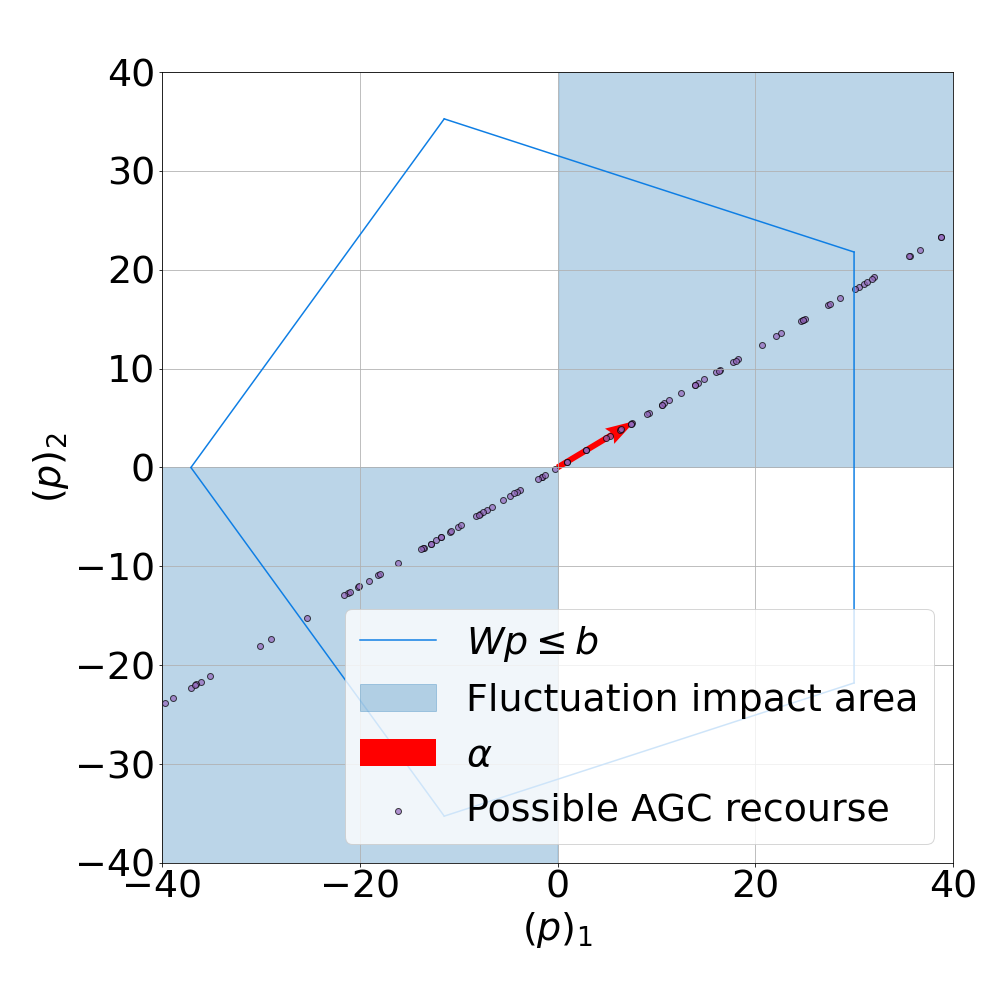
\includegraphics[width=.5\linewidth]{Dissertation/images/dynamic/poly_and_alpha.png}
%     \vspace{-5mm}
%     \caption{The interior of the blue polygon represents the feasibility set, while the brown area represents the possible generation set-points arising from  fluctuations and AGC recourse.
%     } \label{fig:alpha_and_poly}
%     \vspace{-5mm}
% \end{figure}

% \begin{figure}[hbt]
% \vspace{-3mm}
% \begin{subfigure}{.24\textwidth}
%   \centering
%   % include second image
%   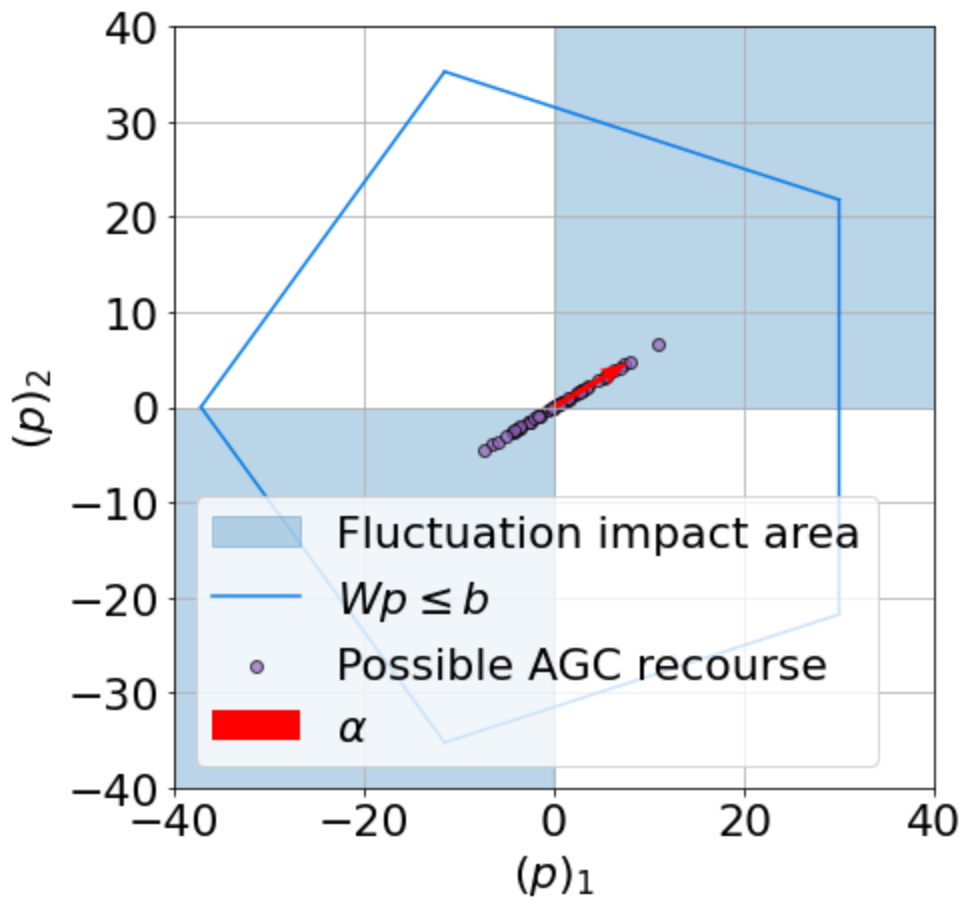
\includegraphics[width=\linewidth]{Dissertation/images/dynamic/recourse_sigma1.png}
%   \caption{Snapshot $t=1$}
%   \label{fig:t=1}
% \end{subfigure}
% % \begin{subfigure}{.24\textwidth}
% %   \centering
% %   % include second image
% %   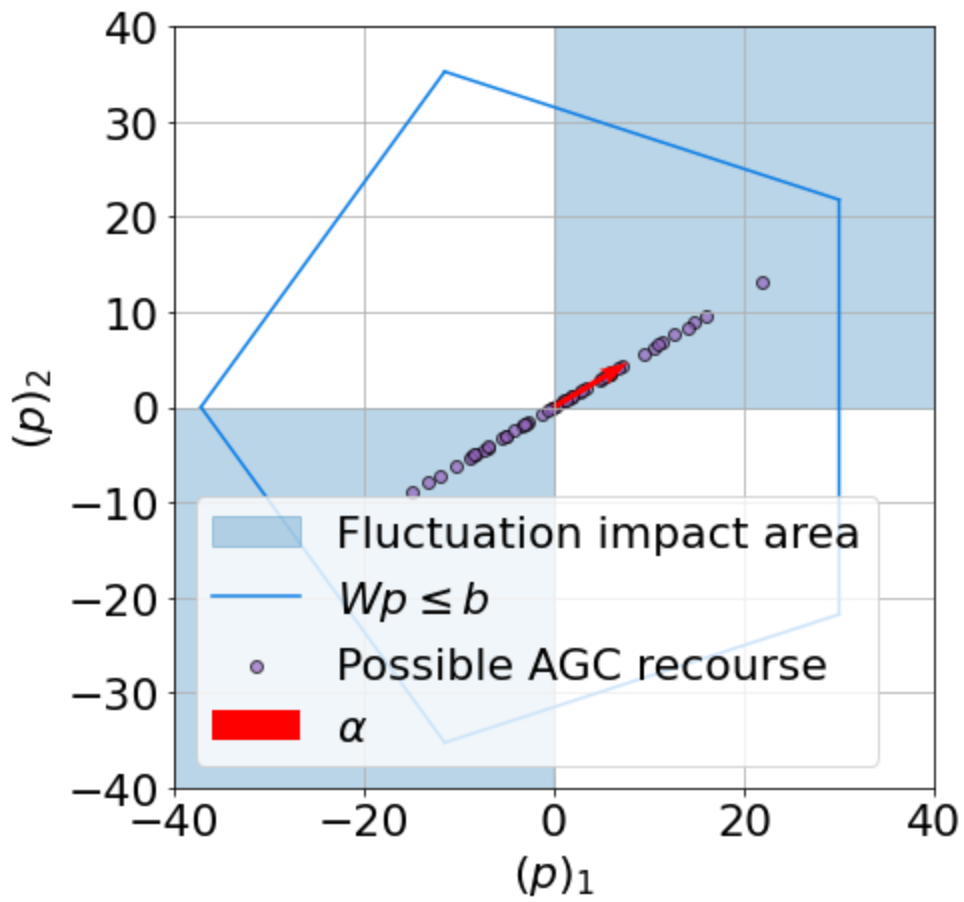
\includegraphics[width=\linewidth]{Dissertation/images/dynamic/recourse_sigma2.png}
% %   \caption{Snapshot $t=2$}
% %   \label{fig:t=2}
% % \end{subfigure}
% % \begin{subfigure}{.24\textwidth}
% %   \centering
% %   % include second image
% %   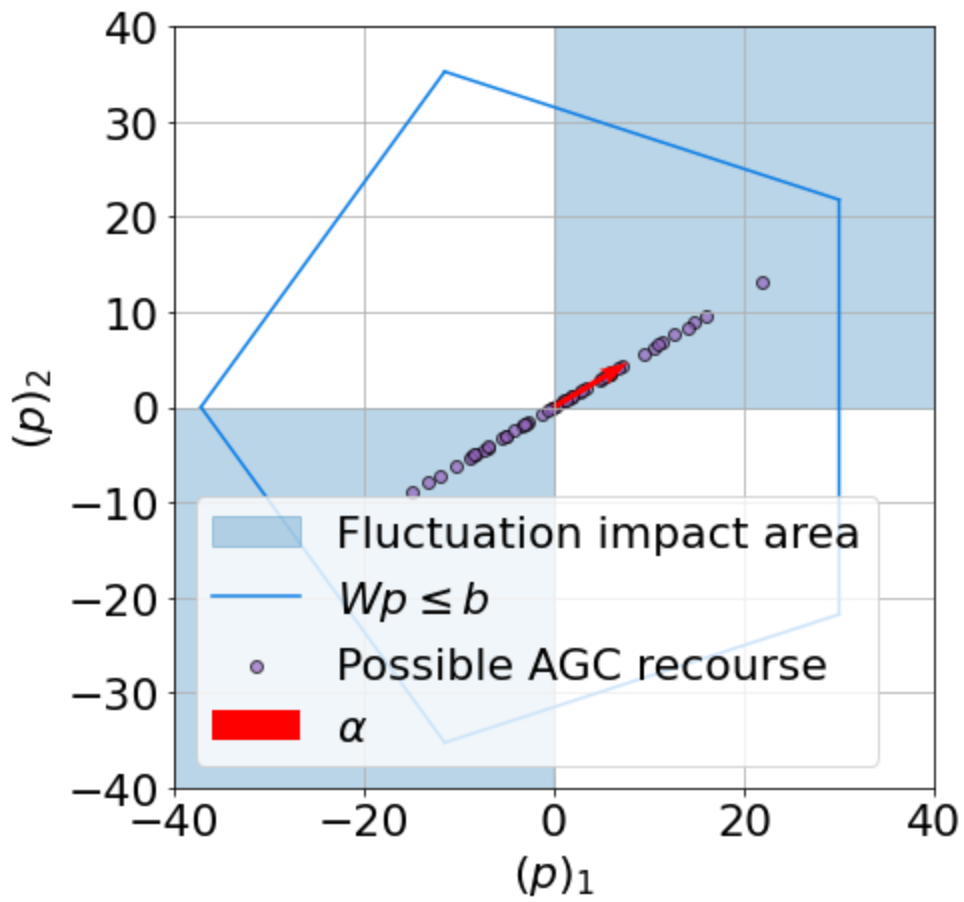
\includegraphics[width=\linewidth]{Dissertation/images/dynamic/recourse_sigma3.png}
% %   \caption{Snapshot $t=3$}
% %   \label{fig:t=3}
% % \end{subfigure}
% \begin{subfigure}{.24\textwidth}
%   \centering
%   % include first image
%   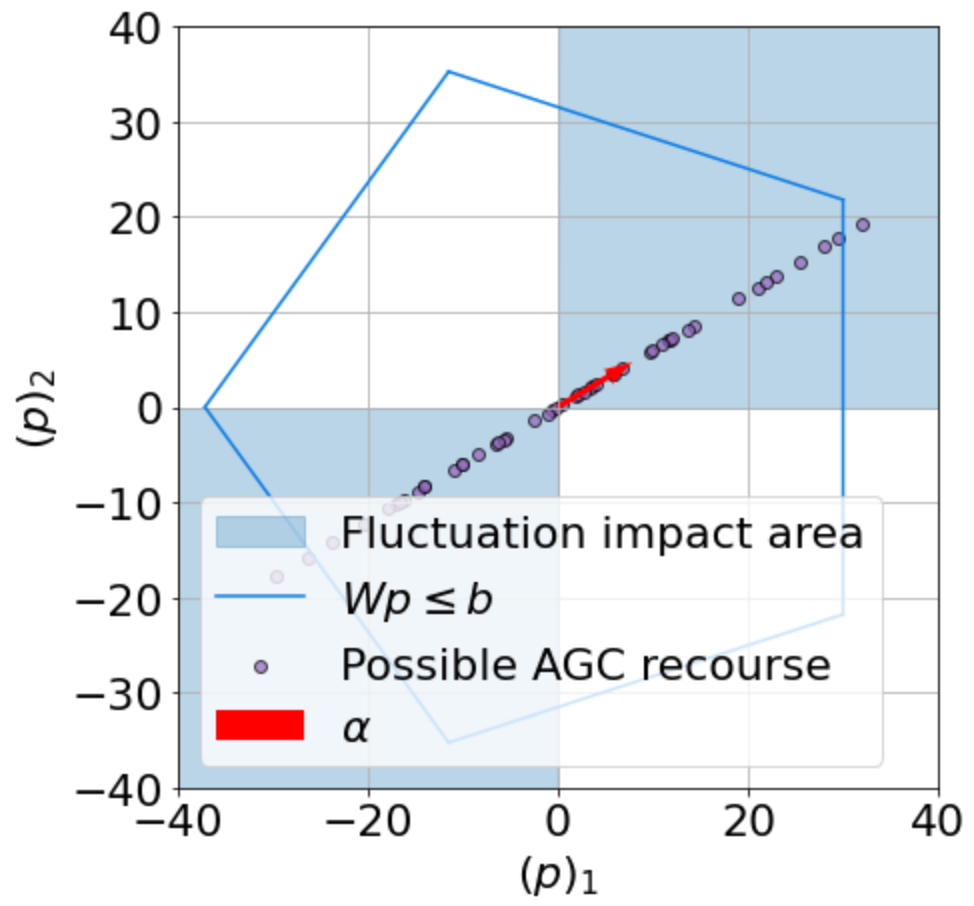
\includegraphics[width=\linewidth]{Dissertation/images/dynamic/recourse_sigma4.png}~~~~~~\hfill
%   \caption{Snapshot $t=4$}
%   \label{fig:t=4}
% \end{subfigure}
% \vspace{-5mm}
% \caption{The growth of variance of total generation demand imbalance $\sum_{\tau \le t}\xi^\tau$ with time $t$.}
% \label{fig:alpha_and_poly_snapshots}
% \end{figure}

Our next step is to derive an upper bound for the failure probability of a control strategy ${(\xi^1, \dots, \xi^T), \alpha}$ with a given starting point $p^0$. 
% To achieve this, we  utilize the following bounds on the probability of $\mathbb{P}(S_1 \cup \dots \cup S_k)$ for some arbitrary sets $S_1, \dots, S_k:$
% \begin{gather*}
%     \max_{i\le k} \mathbb{P}(S_i) \le \mathbb{P}(S_1 \cup \dots \cup S_k) \le \sum_{i\le k} \mathbb{P}(S_i)
% \end{gather*}

%In the context of this chapter, $S_i$ represents the feasibility of the system at $t=i$.
% Notice that as the power system is balanced, we have the following: 
% \begin{gather*}
%     \forall t\le T\quad \sum_{1\le k\le n} p^t_k = 0 \Rightarrow \delta p^t = \sum_{k\le n}\xi^t_k
% \end{gather*}
% thus 
% \begin{gather*}
%     p^t = p^{t-1} + \xi^t - \alpha \sum_{k\le n}\xi^t_k = p^0 + (e-\alpha) \sum_{t\le T}\sum_{k\le n} \xi_k^t, 
% \end{gather*}
% where $e$ is a unit vector, $e = (1, \dots, 1)$. 
% {\color{blue} Sasha, does it match to your equation?}

% The probability that all system states are feasible is given by $\pi = \mathbb{P}\left(\forall k, t:  \omega_k^\top p^t \leq \beta_k, \; k\le n, t\le T\right)$ and must be such as $\pi \geq 1-\eta$.
% Note that $\pi \le 1 -  \max_{k\le n,t\le T}\mathbb{P}(\omega_k^\top p^t > \beta_k)$. Also,  
% $\mathbb{P}\left(\forall i, t: \bigcup_i \omega_i^\top p^t > \beta_i\right) \le 1 -  \max_{i, t}\mathbb{P}(\omega_i^\top p^t > \beta_i)
%     %1 - \mathbb{P}(\omega^\top\sum_{t\le T}\sum_{k\le n} \xi_k^t (1-\alpha_k) < \beta - \omega^\top p^0)\\
%     $
% with $p^t\sim {\cal N}(p^0, \texttt{diag}((\sigma^1)^2, \dots, \sum_{t=1}^{T-1}(\sigma^\tau)^2))$. Now, we have the upper bound $\pi$ greater or equal than $1 - \eta$ we get 
% \begin{equation}
% \max_{i, t}\mathbb{P}(\omega_i^\top p^t > \beta_i) \leq  \eta.
% \label{eq:necessary_JCC}
% \end{equation}
% We use the latter necessary feasibility condition to get the outer approximation of the Joint Chance Constraint (JCC) in Eq.~\eqref{eq:optimal_control_2}.

% We will now derive the \emph{outer} approximation of the JCC (Joint Chance Constraint) feasibility set based on the necessary feasibility condition.
% %It is important to note that if there exists a timestamp $t$ in the range of $1$ to $T$ and a plane $\omega_i$ in the range of $1$ to $J$, such that the necessary feasibility condition \eqref{eq:necessary_JCC} does not hold, it implies that the entire JCC, Prob.~\eqref{eq:optimal_control_2}, cannot be satisfied.
% Assume that for some $t, i$ \eqref{eq:necessary_JCC} is violated.

To get an analytical sufficient condition on the redundant scenarios, we derive a necessary condition for JCC feasibility converted to a sufficient condition of not being in the JCC feasibility set. Note that there is following bound on feasibility probability from \eqref{eq:optimal_control_2}:
\begin{lemma}
    \label{lemma:bound_prob}
     Let $\pi(p^0, \alpha) \geq 1 -\eta$, where $$\pi(p^0, \alpha) = \mathbb{P}\left\{ \cap_{i, \tau} (\omega^p_i)^\top p^0 + (E^\tau_i)^\top \xi \cdot(\omega^\alpha_i)^\top \alpha \leq \beta_i\right\}.$$ Then 
    \vspace{-2mm}
    \[\max_{i, t} \mathbb{P} \left\{ (\omega^p_i)^\top p^0 + (E^\tau_i)^\top \xi \cdot (\omega^\alpha_i)^\top \alpha > \beta_i \right\} \leq 1-\pi(p^0, \alpha).\]
\end{lemma}
\begin{proof}
    As $\mathbb{P}\left\{ \cup_{i, t} (\omega^p_i)^\top p^0 + (E^\tau_i)^\top \xi \cdot (\omega^\alpha_i)^\top \alpha > \beta_i \right\} = 1 - \pi(p^0, \alpha)$, applying the Boole-Fréchet bound \cite[Theorem 4.2.1]{williamson1989probabilistic} to the left-hand side of this we prove the lemma.
\end{proof}
Lemma \ref{lemma:bound_prob} provides a handful necessary condition:
\begin{corollary}
    \label{lemma:corollary}
    Let $(p^0, \alpha)$ be feasible to JCC in \eqref{eq:optimal_control_2}. Then $$\max_{i, t} \mathbb{P} \left\{ (\omega^p_i)^\top p^0 + (E^\tau_i)^\top \xi \cdot (\omega^\alpha_i)^\top \alpha > \beta_i \right\} \leq \eta.$$
\end{corollary}
\begin{proof}
    Feasibility yields $\pi(p^0, \alpha) \geq 1 -\eta$ iff $1 - \pi(p^0, \alpha) \leq \eta$. Applying Lemma \ref{lemma:bound_prob} proves the corollary.
\end{proof}


We now formalize $\hat{\mathcal{P}}_r$ for Problem~\eqref{eq:optimal_control_2}. This gives us a-priori sufficient condition on sample redundancy.

\begin{theorem}
Let scenarios $\xi(j) \sim \mathcal{N}(0, \Sigma), ~ j \in \mathcal{I}=\{1, \dots, N\}$ form SA \eqref{eq:optimal_control_sampling_02} and a solution of this problem $(\hat{p}^0_{\mathcal{I}}, \hat{\alpha}_{\mathcal{I}})$ be feasible for the JCC problem \eqref{eq:optimal_control_2}. Moreover, assume that the cost function $c(\cdot)$ is linear.  Let $\hat{\mathcal{P}}_r = \{ \xi\in \mathbb{R}^T:~ |(E^{\tau}_i)^\top \xi|  \leq \Phi^{-1}(1 - \eta) \sigma^\tau_i \gamma ~\forall i, \tau \}$, where $\gamma \in (0, 1)$ and $(\sigma^\tau_i)^2 = (E^\tau_i)^\top \Sigma (E^\tau_i)$.
Then, first, SA  where scenarios $\xi(j), ~ j \in \mathcal{I}_r = \{ j: \xi(j) \in \hat{\mathcal{P}}_r \}$ yields solution $(\hat{p}^0_{\mathcal{I}_r}, \hat{\alpha}_{\mathcal{I}_r})$ that is not feasible for original JCC Problem \eqref{eq:optimal_control_2}. Second, SA where scenarios $\xi(j), ~ j \in \mathcal{I} \setminus \mathcal{I}_r$ yields the solution $(\hat{p}^0_{\mathcal{I} \setminus \mathcal{I}_r}, \hat{\alpha}_{\mathcal{I} \setminus \mathcal{I}_r})$ that is feasible for the original JCC Problem \eqref{eq:optimal_control_2}.
\label{th:P_r sampling polytope}
\end{theorem}
\begin{proof}
    The feasibility set of SA is given by $(w^p_i)^\top p^0 + (E_i^\tau)^\top \xi(j) \cdot (\omega^\alpha_i)^\top \alpha \leq \beta_i, ~ \forall i, \tau, j$. Since the cost function is linear for solution of SA, $\exists i', \tau', j': ~ (w^p_{i'})^\top p_{\mathcal{I}_r}^0 + (E_{i'}^{\tau'})^\top \xi(j') \cdot (\omega^\alpha_{i'})^\top \alpha_{\mathcal{I}_r} = \beta_{i'}$. Next, one has $(E^{\tau}_i)^\top \xi (j')  \leq \Phi^{-1}(1 - \eta) \sigma^\tau_i \gamma$, because $
    \xi(j') \in \hat{\mathcal{P}}_r$, positive absolute value case. This implies that $(\omega^p_{i'})^\top p^0_{\mathcal{I}_r} \geq \beta_{i'} - \Phi^{-1}(1-\eta) \sigma^{\tau'}_{i'} \| (\omega_{i'}^\alpha)^\top \alpha_{\mathcal{I}_r} \| \gamma$. However, the necessary condition from Corollary \ref{lemma:corollary} implies that $\forall i, \tau ~ (\omega_i^p)^\top p^0_{\mathcal{I}_r} \leq \beta_i - \Phi^{-1}(1-\eta) \sigma^\tau_i \| (\omega_i^\alpha)^\top\alpha_{\mathcal{I}_r}\|$. Recalling that $\gamma \in (0, 1)$ we obtain contradiction that leads to the fact that $(\hat{p}_{\mathcal{I}_r}^0, \hat{\alpha}_{\mathcal{I}_r})$ is infeasible for original JCC Problem.
    Now drop redundant scenarios from the SA. Since $(\hat{p}^0_{\mathcal{I}}, \hat{\alpha}_{\mathcal{I}})$ is feasible for JCC problem and data samples $\xi(j), ~ j \in \mathcal{I}_r$ do not contribute to the feasibility, then SA solution $(\hat{p}_{\mathcal{I} \setminus \mathcal{I}_r}^0, \hat{\alpha}_{\mathcal{I} \setminus \mathcal{I}_r})$ built on $\xi(j), ~ j \in \mathcal{I} \setminus \mathcal{I}_r$ is feasible for JCC problem.
\end{proof}

\begin{comment}
{\color{orange}
\begin{theorem}[NVC - Necessary Violation Criterion]
    \label{th:NVC}
    Let $p^0 \in \mathbb{R}^{n_g}, \alpha \in \mathbb{R}^{n_g}$. A pair $p^0, ~ \alpha$ does not satisfy $\max_{i, t} \mathbb{P} \left\{ \omega^\top_i p^t > \beta_i \right\} \leq \eta$ $\iff$ $\exists i, t, \omega_i^\top \alpha \neq 0: ~ \omega_i^\top p^0  > \beta_i - \Phi^{-1}(1-\eta)\tilde{\sigma}^t \| \omega_i^\top \alpha \|$, where $\Phi(\cdot)$ is a CDF of standard normal Gaussian r.v. 
\end{theorem}
\begin{proof}
    A pair $p^0, ~\alpha$ does not satisfy $\max_{i, t} \mathbb{P} \left\{ \omega^\top_i p^t > \beta_i \right\} \leq \eta$ $\iff$ $\exists i, t, \omega_i^\top \alpha \neq 0: ~ \mathbb{P}\left\{ \omega^\top_i p^0 + \omega_i^\top \alpha \zeta^t > \beta_i \right\} > \eta$. The latter is equivalent to $\Phi\left( \frac{\omega_i^\top p^0}{\tilde{\sigma}^t \| \omega_i^\top \alpha \|} \right) > \eta$, which, due to the monotonicity of the CDF, can be setup as $\omega_i^\top > \beta_i - \Phi^{-1}(1 - \eta) \tilde{\sigma}^t \| \omega_i^\top \alpha \|$.
\end{proof}
Based on violation criteria \ref{th:NVC} we present formal description of scenario necessarial non-redundancy.
\begin{definition}
    \label{def:necessary_non-redundant}
    Let SA \eqref{eq:optimal_control_sampling_02} be based on scenarios $\xi^t(j), ~ j \in \mathcal{I} = \{1, \dots, N \}$. Scenarios indexed with $\mathcal{I}_{NNR},~ \mathcal{I}_{NNR} \subset \mathcal{I}$ are called Necessarily Non-Redundant (NNR) $\iff$  $\forall i,~ \forall j \in \mathcal{I}_{NNR}$ $\sign(\omega_i^\top \alpha) \zeta^t (j) > \Phi^{-1}(1 - \eta) \tilde{\sigma}^t $.
\end{definition}
\begin{definition}
    \label{def:sufficiently_redundant}
    Let SA \eqref{eq:optimal_control_sampling_02} be based on scenarios $\xi^t(j), ~ j \in \mathcal{I} = \{1, \dots, N \}$. Scenarios indexed with $\mathcal{I}_{SR},~ \mathcal{I}_{SR} \subset \mathcal{I}$ are called Sufficiently Redundant (SR) $\iff$  $\forall i,~ \forall j \in \mathcal{I}_{SR}$ $\sign(\omega_i^\top \alpha) \zeta^t (j) < \Phi^{-1}(1 - \eta) \tilde{\sigma}^t \gamma $, where $\gamma = \min_{i, ~\alpha: \|\alpha - \alpha_0\|_2 \leq \delta \alpha, ~ \omega_i^\top \alpha \neq 0} \| \omega_i^\top \alpha \|.$
\end{definition}
Evidently, a scenario cannot be simultaneously NNR and SR.
The next theorem reveals the purpose of the definitions above and allows one to classify scenarios based on redundancy.
\begin{theorem}
    \label{th:redundancy_classify}
    Let SA \eqref{eq:optimal_control_sampling_02} be based on scenarios $\xi^t(j), ~ j \in \mathcal{I} = \{1, \dots, N \}$. Also, let $c(p^t)$ be linear and the solution of SA with scenarios $\mathcal{I}$ $(\hat{p}^0, \hat{\alpha})$ be feasible for JCC. Then, SR scenarios with indexes $\mathcal{I}_{SR}$ are redundant.
\end{theorem}
\begin{proof}
    Let us consider SA built only on SR scenarios. This yields that the solution of such scenario approx $(\hat{p}^0_{\mathcal{I}_{SR}}, \hat{\alpha}_{\mathcal{I}_{SR}}).$ Due to the  From the definition of SR scenarios, we have that $\omega^\top_i \hat{p^0} \leq \beta_i - \Phi^{-1}(1-\eta) \tilde{\sigma}^t \gamma ~ \forall ~i, t$. Moreover, due to the linearity of the cost function, $\exists k, j: \omega_k^\top \hat{p}^0 = \beta_k - \omega_k^\top \alpha \zeta^t(j)$. Since $\zeta^t(j)$ is a SR scenario and $\sign(x) = x / \|x\|, ~ x \neq 0$, one obtains,  $\omega_k^\top \hat{p}^0 \geq \beta_i - \Phi^{-1}(1-\eta)\tilde{\sigma}^t \gamma$ for this constraint. Moreover, since $\gamma \leq \| \omega_k^\top \alpha \|$, one obtains $\omega_k^\top \hat{p}^0 \geq \beta_i - \Phi^{-1}(1-\eta)\tilde{\sigma}^t \| \omega_k \alpha \|$. Using Th. \ref{th:NVC} and Corollary \ref{lemma:corollary} one obtains that those scenarios lead to infeasible, for JCC, solution. So, each NR scenario is redundant by definition.
\end{proof}
}
\end{comment}
\begin{comment}
{\color{orange}
Moreover, right-hand sides of the inequalities decrease from deterministic $\beta_i$ as $\tilde{\sigma}^t = \sqrt{\sum_{\tau=1}^{t-1} (\sigma^\tau)^2}$ grows. Figure~\ref{fig:evoluted} illustrates the mutual geometry between initial feasibility polytope and necessary feasibility polytope at $t > 1$. It's worth noting that since $\Delta_i^t$ depends on $| \omega_i^\top \alpha |$, the planes that are closer to being orthogonal to the participation vector $\alpha$ are less impacted by the uncertainty in control policy.
}
\end{comment}
%In other words, such planes of $\mathcal{P}_{out}$ have slower decreasing right hand side.
% \begin{remark}
% Additionally, the same reasoning applies to the ramp-up and ramp-down constraints $|\alpha_k \xi^t| \leq R_k$. In this case, the logic remains unchanged for the hyperplanes $\alpha_i\xi^t \leq R_i$. It's important to note that $|\alpha_k \xi^t| \leq R_k$ is equivalent to the simultaneous satisfaction of $\alpha_k \xi^t \leq R_k$ and $-\alpha_k \xi^t \leq R_k$.
% \end{remark}
\begin{comment}
\begin{figure}
    \begin{subfigure}{.24\textwidth}
        \centering
        % \vspace{-3mm}
        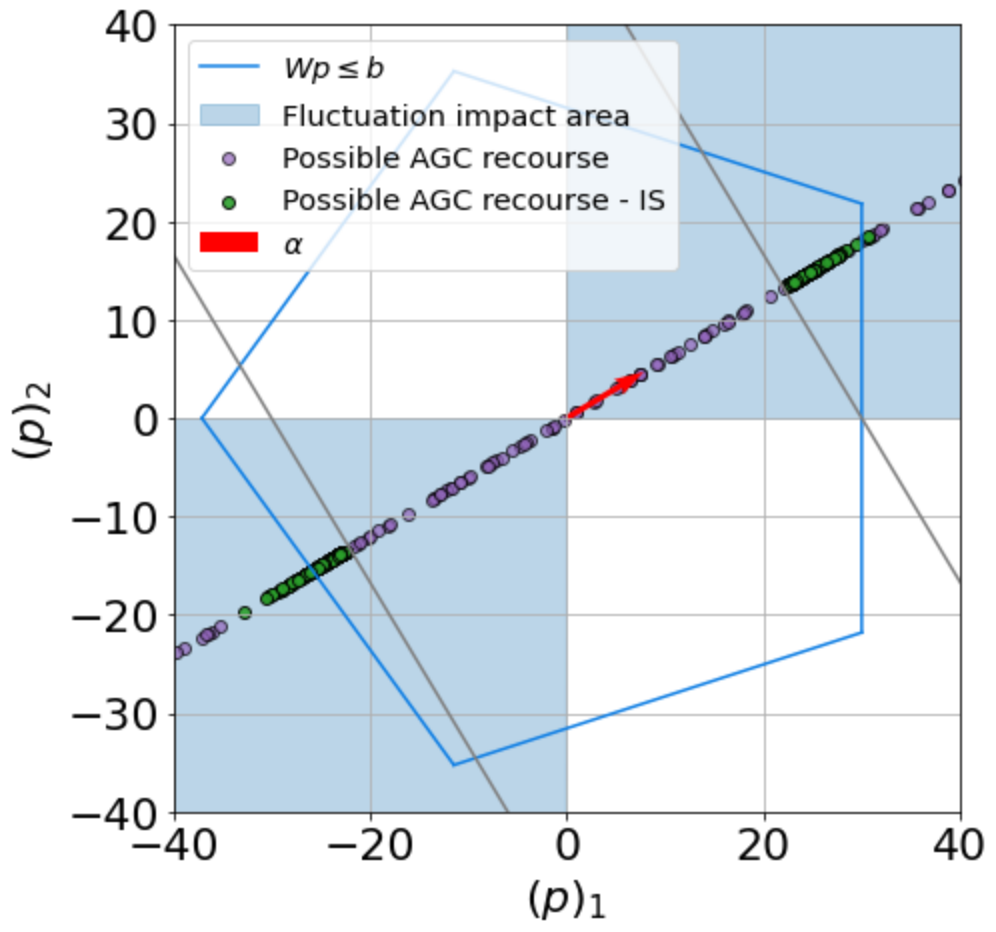
\includegraphics[width=.8\textwidth]{Dissertation/images/dynamic/poly_and_alpha_mc_vs_is.png}
        \vspace{-2mm}
        \caption{AGC recourses from non-redundant sample set $\mathcal{P}_r$ that lead to violation of technical limits.
        }
        \label{fig:importance_sampled_vs_mc}
        \vspace{-5mm}
    \end{subfigure}
    \begin{subfigure}{.24\textwidth}
        \centering
        \vspace{-3mm}
        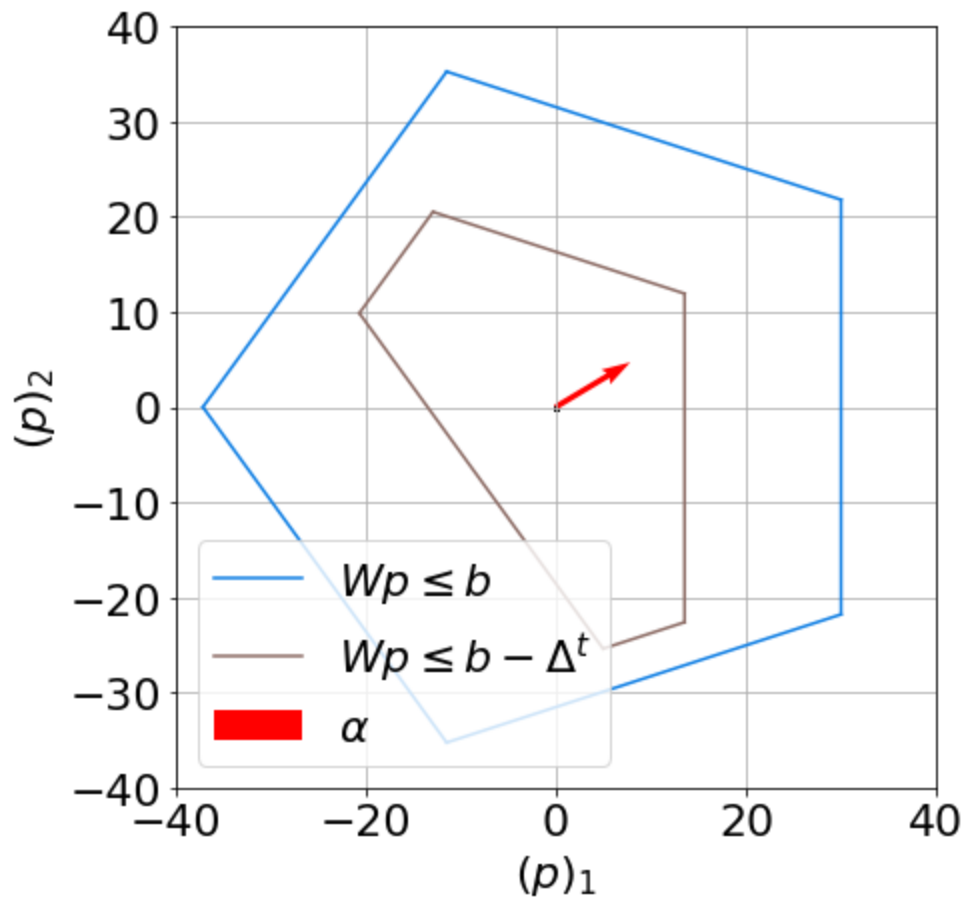
\includegraphics[width=.8\textwidth]{Dissertation/images/dynamic/necessary_poly.png}
        \vspace{-2mm}
        \caption{Mutual position of the deterministic feasibility polygon $Wp_g \leq b$ and $\mathcal{P}_{out}$. }
        \label{fig:evoluted}
        \vspace{-5mm}
    \end{subfigure}
    \label{fig:demo}
    \caption{\color{orange} The impact of uncertainty on feasibility sets and AGC.}
    \vspace{-4mm}
\end{figure}
\end{comment}
Theorem \ref{th:P_r sampling polytope} establishes a sufficient, i.e., a priori condition on sample redundancy across a given dataset $\xi(j), j \in \mathcal{I}$ that guarantees a feasible solution. Specifically, if a dataset provides assurance of producing a feasible solution for the original JCC problem, samples within $\hat{\mathcal{P}}_r$ may be disregarded. Thus this theorem offers a way to assess the dataset's potential a-priori: if all data samples fall within $\mathcal{P}_r$, it is be impossible to derive any feasible solution for the JCC from this data.
%$\zeta(j) = (\zeta^1(j),\dots, \zeta^T(j)) \sim \mathcal{N}(0, \Sigma_{\zeta})$ outside of the polytope $\underline{P}_{r} = \left\{ (\zeta^1, \dots, \zeta^T)^\top: ~ \omega_i^\top \alpha \zeta \leq \Phi^{-1}(1 - \eta) \| \omega_i^\top \| \tilde{\sigma}^t \gamma , ~ \forall~ t,~ \forall~ i\right\}$ to increase data efficiency of the SA. 
%{\color{red} Should I delete this?}
%{ \color{gray}
%The polytope can equally be described as $\mathcal{P}_{r} = \left\{ \mathbf{\zeta}: ~ \mathcal{W} \mathbf{\zeta} \leq \Phi^{-1}(1-\eta) \mathcal{S}\right\}$. 
%Here $\mathcal{W} \in \mathbb{R}^{(J \cdot T) + (2 \cdot n_g \cdot T)\times T}$ is a block diagonal matrix. The $j^{\textup{th}}$ block of the matrix is of a shape $T \times T$ and $\mathcal{W}_j =  \sign(\omega_k^\top \alpha) \cdot I$ where $j \in 1 + (k - 1) \cdot T, \dots, k \cdot T $, $k=1, \dots, J$. The other blocks correspond to the ramp-up/down constraints. They are as follows: $\mathcal{W}_j=I$ for $j\in J\cdot T + 1 + (k-1) \cdot T, \dots J\cdot T + 1 + k \cdot T$ and $k=1, \dots, n_g$. The remaining blocks of the matrix are the same except the sign and correspond to the ramp-down constraints. The vector on right-hand side is $\mathcal{S} = (\mathcal{S}_{\mathcal{W}}, \mathcal{S}_{ramp})$, where $\mathcal{S}_{\mathcal{W}}= (\tilde{\sigma}^1, \dots, \tilde{\sigma}^T, \dots,  \tilde{\sigma}^1, \dots, \tilde{\sigma}^T)$ and 
%\[\mathcal{S}_{ramp} =\left[\frac{R_1}{\alpha_1 \sigma^1}, \dots, \frac{R_{n_g}}{\alpha_{n_g} \sigma^1}, \dots,
%\frac{R_1}{\alpha_1 \sigma^T}, \dots, \frac{R_{n_g}}{\alpha_{n_g} \sigma^T}\right].\] 
%Overall, $ \mathcal{S} \in \mathbb{R}^{J \cdot T + 2 \cdot n_g \cdot T}$.
%}
%{\color{red} Should I delete this?}

%\vspace{-4mm}
\subsection{SA Solution Guarantees and Dataset Complexity}
In this section we provide theoretical guarantees on the solution of reduced SA that does not contain redundant samples within $\hat{\mathcal{P}}_r$.
The following theorem addresses the sampling complexity of the SA with data samples indexed $\mathcal{I} \setminus \mathcal{I}_r$.
\begin{theorem}\label{thm:40}
Let $(\hat{p}^0, \hat{\alpha})$ be a unique solution of the SA Problem~\eqref{eq:optimal_control_sampling_02} with $N$ i.i.d. samples, so that none of the samples belong to $\hat{\mathcal{P}}_{r}$. Moreover, assume that for any $N$ the assumption \ref{asmp:10} is fulfilled. Then for any $\rho \in (0,1)$ and any~$\eta \in (0, 1/2]$, $(\hat{p}^0, \hat{\alpha})$ is also a solution for the Chance-constrained optimal power flow Problem~\eqref{eq:optimal_control_2} with probability at least $1-\rho$ if 
$%\begin{align*}
  N \ge \left\lceil 2\eta^{-1}(1-\nu)\ln \frac{1}{\rho} + 2d + 2d\eta^{-1}(1-\nu) \ln\frac{2(1-\nu)}{\eta} \right\rceil, 
$%\end{align*} 
 where $d$ is a dimension of the space of controllable generators and participation factors, i.e., $d = 2 n_g$, and $\nu$ is the probability of a random scenario $\xi \sim \mathcal{N}(0, \Sigma)$ to belong to $\hat{\mathcal{P}}_{r}$, and $\nu < 1$. 
\end{theorem}
\begin{proof}
First, notice that discarding random scenarios $\xi \notin \hat{\mathcal{P}}_{r}$ is equivalent in solving the SA problem with sampling 
$\xi$ from a distribution $\mathcal{D}$ where  
$\xi \sim \mathcal{D} \Leftrightarrow \xi\sim \mathcal{N}(0, \Sigma) \textup{s. t. } \xi\not\in \hat{\mathcal{P}}_{r}$. 
From the theorem statement, $1-\nu$ is the probability mass associated with samples in $\xi\sim \mathcal{N}(0, \Sigma)$ 
that are outside $\hat{\mathcal{P}}_{r}$.
%
 Assumption \ref{asmp:10} and convexity of each function in Problem \ref{eq:optimal_control_2} meet the conditions of Calafiori and Campi~\cite[Theorem 1]{calafiore2006scenario} implying that for any probability $\rho \in (0,1)$ and any confidence threshold probability $\varepsilon$, and dimension of the space of parameters $d$ one has, for~$N_1$
\vspace{-1mm}
\begin{align}\label{eq:mon}
\vspace{-2mm}
  N_1 \ge \left\lceil 2\varepsilon^{-1} \ln (1/\rho) + 2d + 2d\varepsilon^{-1} \ln (2/\varepsilon)\right\rceil 
\end{align}
%\vspace{-1mm}
scenarios from $D$ and the optimal solution 
$(\hat{p}^0, \hat{\alpha})$ of the Problem~\eqref{eq:optimal_control_sampling_02}, 
%(\textcolor{red}{or (9)?})
the probability of failure is bounded as $
  \mathbb{P}_D\{(\hat{p}^0, \hat{\alpha}) \textup{ is feasible for \ref{eq:optimal_control_2}}\} \geq 1-\varepsilon
$ with prob. at least $1-\rho$. 

Notice, that the bounds on the number of samples (see Eq.~\eqref{eq:mon}) is strictly decreasing in $\varepsilon$ for $\varepsilon \in (0,1)$. As scenarios in $\hat{\mathcal{P}}_{r}$ are redundant and do not contribute to overall solution reliability, to get a probability of failure $\eta$ according to measure $\mathcal{N}(0, \Sigma)$, we need the failure probability according to $\mathcal{D}$ to be at least $\varepsilon = \eta/(1-\nu)$.  
Thus, using $\varepsilon = \eta/(1-\nu)$ and monotonicity of~Ineq.~\eqref{eq:mon} one completes the proof. 
\end{proof}


% Although, in practice, it is impossible to draw samples from $\mathcal{D}$. Thus, the next subsection is devoted to practical sampling form mixture and theoretical implications of it.


%$$
%\begin{aligned}
%\mathbb{P}\Big( (p_0, \alpha) \in \mathcal{P} \Big)&=\mathbb{P}\Big( \mathcal{W}^p p_0 + \mathcal{W}^{\alpha} \alpha \circ \Pi \vec{\xi} \leq \beta \Big) =\\
%&\mathbb{P}\Big( \cap_{i=1}^{J}\mathcal{W}^p_i p_0 + \mathcal{W}^{\alpha}_i \alpha \circ \Pi_i \vec{\xi} \leq \beta_i \Big) =\\
%&1 - \mathbb{P}\Big( \cup_{i=1}^{J}\mathcal{W}^p_i p_0 + \mathcal{W}^{\alpha}_i \alpha \circ \Pi_i \vec{\xi} > \beta_i \Big) \leq\\
%&1 - \max_{i=1, \dots,J}\mathbb{P}\Big( \mathcal{W}^p_i p_0 + \mathcal{W}^{\alpha}_i \alpha \circ \Pi_i \vec{\xi} > \beta_i \Big)
%\end{aligned}
%$$
% One can see that if there is a plane $i$ that for some initial generation set-point $p_0$ and participation factors $\alpha$ such that $\mathbb{P}\Big( \mathcal{W}^p_i p_0 + \mathcal{W}^{\alpha}_i \alpha \circ \Pi_i \vec{\xi} > \beta_i \Big) > \eta$ then the whole JCC has probability less than $1-\eta$ to satisfy, making this a necessary condition for JCC feasibility. On the other hand, the fact that $\max_{i=1, \dots,J}\mathbb{P}\Big( \mathcal{W}^p_i p_0 + \mathcal{W}^{\alpha}_i \alpha \circ \Pi_i \vec{\xi} > \beta_i \Big) \leq \eta$ does not mean that JCC is satisfied, thus, it is not sufficient feasibility condition. 
% Nevertheless, we will use this necessary condition to construct \emph{outer} approximation of $\mathcal{F}$, which will turn out to be inner approximation of deterministic polytope under probability. Using that, we will define which scenarios can be dropped from the scenario approximation without any consequence, i.e., \emph{redundant} scenarios.
% Thus, to satisfy the necessary condition, current operating point should satisfy. Denoting $\Sigma^{1/2} = \texttt{diag}(\sigma_1, \dots, \sigma_T)$
% $$
% \begin{aligned}
% \eta &\geq \mathbb{P}\Big( \mathcal{W}^p_i p_0 + \mathcal{W}^{\alpha}_i \alpha \circ \Pi_i \vec{\xi} > \beta_i \Big) =\\
% &\mathbb{P}\Big( \frac{\mathcal{W}^{\alpha}_i \alpha \circ \Pi_i \vec{\xi}}{\| \Sigma^{1/2} \mathcal{W}^{\alpha}_i \alpha \circ \Pi_i \|} >\frac{\beta_i - \mathcal{W}^p_i p_0}{\| \Sigma^{1/2} \mathcal{W}^{\alpha}_i \alpha \circ \Pi_i \|} \Big) =\\
% &\Phi\left( \frac{\beta_i - \mathcal{W}^p_i p_0}{\| \Sigma^{1/2} \mathcal{W}^{\alpha}_i \alpha \circ \Pi_i \|} \Big) \right)
% \end{aligned}
% $$
% Here $\Phi$ is the cdf of standard normal distribution. The condition can be reformulated in terms of the following set:
% $\mathcal{P}_{in} = \{ (p_0, \alpha): \mathcal{W}^p_i p_0 \leq \beta_i - \Phi^{-1}(1-\eta) \| \Sigma^{1/2} \mathcal{W}^\alpha_i \alpha \circ \Pi_i\|\}$. One can observe that for fixed $\alpha = \alpha_0$ this set is the polytope in $p_0$ (initial generation set-point) that defines inner approximation for feasibility set.
% %To define a condition on sample redundancy one must consider inner approximation of non-convex chance-constrain feasibility set. This is easily achieved if one considers Single Chance Constraint (SCC) formulation instead of more accurate Joint Chance Constraint (JCC) as in Problem \ref{eq:optimal_control_1}.
% %The SCC is built from the constraints of the following form: $\mathbb{P} (\omega_i^\top p_0 > b_i - \omega_i^\top \alpha_0 \xi_t) \leq 1 - \eta$. One may rewrite is at $\mathbb{P}\left( \textup{sign}(\omega_i^\top \alpha_0) \xi_t / \sigma_t > \frac{b_i - \omega_i^\top p_0}{|\omega_i^\top \alpha_0|} \right) < \eta$, which is equivalent to $w_i^\top p_0 \leq b_i - \Phi^{-1}(1 - \eta) \sigma_t |\omega_i^\top \alpha_0| $. If one brings the stochastic part back into this constraint, one would obtain $w_i^\top p_0 + \omega_i^\top \alpha_0 \xi_t \leq b_i + \Phi^{-1}(1 - \eta) \sigma_t |\omega_i^\top \alpha_0| $. From here it is evident that if $\xi_t$ is such that $\omega_i^\top \alpha_0 \xi_t \leq \Phi^{-1}(1 - \eta) \sigma_t |\omega_i^\top \alpha_0|$ then $p_0$ satisfies this constraint. Next, one can construct a polytope for realization $\xi_\tau, ~ \tau=1, \dots, T$ -- the trajectories of disturbances that would lead to no violation of constraints. Next, considering only those samples that are out of it, a more efficient scenario approximation is constructed. Let us denote this polytope as $\mathcal{P}_0 = \Big\{ (\xi^1, \dots, \xi^T):~ \omega_i^\top \alpha_0 \xi_t \leq \Phi^{-1}(1 - \eta) \sigma_t |\omega_i^\top \alpha_0|,$ $t=1, \dots, T, ~ i=1, \dots, m  \Big\}$.
% {\color{red} Now we discuss the process of sampling non-redundant scenarios. Let us consider AGC recourse differences for $T$ snapshots and its effect due to a realization of perturbation $\vec{\xi}^i$ and compare it to the necessity fix given by }
% \begin{equation}
%     \mathcal{W}_i \alpha \circ \Pi_i \vec{\xi}^i - \Phi^{-1}(1 - \eta) \| \Sigma^{1/2} \mathcal{W}^\alpha_i \alpha_0 \circ \Pi_i \|.
%     \label{eq:sample_redundancy}
% \end{equation} {\color{red} If this difference is non-negative then one would obtain that the scenario $\vec{\xi}^i$ does not drive generation set-point sequence out of the feasibility region contributing none to the infeasibility modeling which is essential for construction of scenario spproximation. Otherwise, it does. Thus, the condition of sample redundancy is given by eq. \ref{eq:sample_redundancy}. The scenario approximation should be constructed with samples drawn outside of this polytope $\mathcal{P}_0$.}
% % Now we discuss the process of sampling of productive scenarios. The goal is to obtain samples $(\xi^1, \dots, \xi^T)_i$ that lie out of $\mathcal{P}_0$. Let us consider $T$ snapshots and assume that $\xi_\tau \sim \mathcal{N}(0, \sigma^2_\tau)$. Note that both the initial generation set-point and AGC recourse must satisfy feasibility constraints. One can write these constraints in a compact notation: $\mathbb{P}\left(W_T p_0 + W_T\alpha \circ \Pi_T \vec{\xi} \leq b_T\right) \geq 1-\eta$. 
% % Thus, $\mathcal{P}_0$ can be equivalently defined as $\mathcal{P}_0 = \Big\{ \vec{\xi}:~ (W_T \alpha_0 \circ \Pi_T) \vec{\xi} \leq \Phi^{-1}(1 - \eta) |W_T \alpha_0| \circ \Pi_T \cdot (\sigma_1, \dots \sigma_T)^\top  \Big\}$. 
% % Sampling realizations of random vectors out of $\mathbb{P}_0$ can be conducted using ALOE {\color{red} cite MC} algorithm. ALOE allows one to obtain samples that are conditioned to be located of the polytope specified. In our case, we choose $\mathcal{P}_0$ to sample out of. In other words, we sample realizations of $\vec{\xi} \sim D_{\mathcal{P}_0}$, where $D_{\mathcal{P}_0} \sim \mathcal{N}(0, \texttt{diag}(\sigma_1^2, \dots, \sigma_T^2), ~ \vec{\xi} \notin \mathcal{P}_0$.
%\vspace{-3mm}
% START OF SAMPLING
\begin{comment}
\subsection{Sampling non-redundant scenarios}
\label{sec:sampling}

In order to sample non-redundant scenarios, we approximate their distribution with a distribution mixture $D$ that has the density $f_D(x) = \sum_{i=1}^{|\mathcal{S}|}w_i f_{D_i} (x).$ Here $|\mathcal{S}| = J \cdot T + 2 \cdot n_g \cdot T$, mixture components' weights are positive and $\sum_{i} w_i  = 1$, $f_{D_i}$ are mixture components densities. The mixture components are Gaussians conditioned on a single linear constraint's complement. For a plane $i$: $\xi \sim D_i \Longleftrightarrow \mathcal{N}(0, \Sigma), ~ \mathcal{W}_i^\top x > \mathcal{S}_i$. The exact expression for the density is $f_{D_i} = \textbf{1} (\mathcal{W}_i^\top x > \mathcal{S}_i) f(x) / \mathbb{P}(\mathcal{W}_i^\top x > \mathcal{S}_i)$, where the probability also has explicit expression: $\mathbb{P}(\mathcal{W}_i^\top x > \mathcal{S}_i) = \Phi(-\mathcal{S}_i / \| \Sigma^{1/2}_{\zeta} \mathcal{W}_{i} \|)$. Such mixture has proven to be useful in approximating the distribution of interest \cite{lukashevich2021importance}, \cite{lukashevich2021power}, \cite{owen2019importance}. For this study, we use $w_1 = \dots = w_{|\mathcal{S}|}$.

In order to sample from this mixture, one must pick a plane with probability $w_i$ and then sample outside of this plane.
The Algorithm \ref{alg:sample1d} summarizes the procedure to produce samples outside of a plane of $\mathcal{P}_r = \{ \xi\in \mathbb{R}^T:~ (E^{\tau}_i)^\top \xi \cdot \sign[ (\omega^{\alpha}_i)^\top \alpha] \leq \Phi^{-1}(1 - \eta) \sigma^\tau_i \gamma ~\forall i, \tau \}$. 
\begin{algorithm}[H]
 \caption{Sampling $\xi \sim\mathcal{N}(\mu,\Sigma)$ s.t. $\xi^\top \omega_i \geq b_i$}
 \label{alg:sample1d}
 \begin{algorithmic}[1]
 \renewcommand{\algorithmicrequire}{\textbf{Input:}
 }
 \Require Mean $\mu$, covariance $\Sigma$, and a constraint $p^\top \omega^i \le b_i$.
 \renewcommand{\algorithmicensure}{\textbf{Output:}}
 \Ensure  $p\sim\mathcal{N}(\mu,\Sigma)$ s.t. $p^\top \omega^i \ge b_i$
 %\\ \textit{Initialisation}: 
  \State  Sample $z \sim \mathcal{N}(0, I_n)$ and $u \sim U(0,1)$
  \State  Compute $y = \Phi^{-1}(\Phi(\tau) + u(1 - \Phi(\tau)))$
  \State Set $\phi = \bar\phi y + (I_n - \bar\phi\phi^\top) z$, with $\bar\phi = \Sigma^{1/2} \omega^i / \|\Sigma^{1/2} \omega^i\|_2$\!\!
  \Return $p = \Sigma^{1/2} (\phi+\mu)$
 \end{algorithmic}
 \end{algorithm}

With given samples $\xi^t(j)$ where $j=1, \dots, N$ and $t=1, \dots, T$, we can now construct the scenario approximation \ref{eq:optimal_control_sampling_02}. Figure \ref{fig:importance_sampled_vs_mc} shows the difference between the samples obtained from the importance sampling procedure described above and the classical Monte Carlo (MC) approach as a sampler.

To analyze the sampling complexity using this proxy distribution, one needs to figure out the interrelation between density of proxy distribution and exact distribution that is Gaussian without $\mathcal{P}_r$. From \cite{lukashevich2021power} one has:

\begin{theorem}\label{thm:50}
Let $q_D(x)$, $f_D(x)$ be PDFs  of $\xi \sim\mathcal{N}(0, \Sigma) \st \xi\not\in\mathcal{P}_{r}$, and a mixture density resp. Then for any $\xi\not\in\mathcal{P}_{r}$, we have
\begin{align}\label{eq:M}
  q_D(\xi) \le M f_D(\xi),  
  M = \frac{\sum_{i\le J} \Phi(-\Delta_i/\|\Sigma^{1/2}\omega_i\|_2)
  }{\max_{i\le J}\Phi(-\Delta_i/\|\Sigma^{1/2}\omega_i\|_2)}.
\end{align}
\end{theorem}

Having the interrelation between densities, we can now prove the sampling complexity of SA based on proxy mixture:
\begin{theorem}\label{thm:80}
Let $(\hat{p}^0, \hat{\alpha})$ be a unique solution of the SA Problem~\eqref{eq:optimal_control_sampling_02} with $N$ i.i.d. samples follow mixture distribution$D$. Moreover, assume that for any $N$ the assumption \ref{asmp:10} is fulfilled. Then for any $\rho \in (0,1)$ and any~$\eta \in (0, 1/2]$, $(\hat{p}^0, \hat{\alpha})$ is also a solution for the chance-constrained optimal power flow Problem~\eqref{eq:optimal_control_2} with probability at least $1-\rho$ if 
\begin{align*}
  N \ge \left\lceil Z\ln \rho^{-1} + 2d + d Z\ln Z \right\rceil, 
\end{align*} 
where $Z = 2M\eta^{-1}(1-\nu)$, $d$ is a dimension of the problem and $\nu$ is a probability of a random scenario $\zeta$ to belong to $\mathcal{P}_{r}$, $\nu < 1$, and constant $M$ is defined by Theorem~\ref{thm:50}.
\end{theorem}
\begin{proof}
The proof is similar to the one of Theorem~\ref{thm:40}. Application of theorem \ref{thm:50} allows to upper-bound the probability of an event in measure $D$ with respect to its probability in measure $\mathcal{N}(0,\Sigma_{\zeta}) \st \zeta\not\in\mathcal{P}_{r}$. 
\end{proof}
\end{comment}
% END OF SAMPLING
%\vspace{-1mm}
%  \begin{figure}
%     \centering
%     \vspace{-3mm}
%     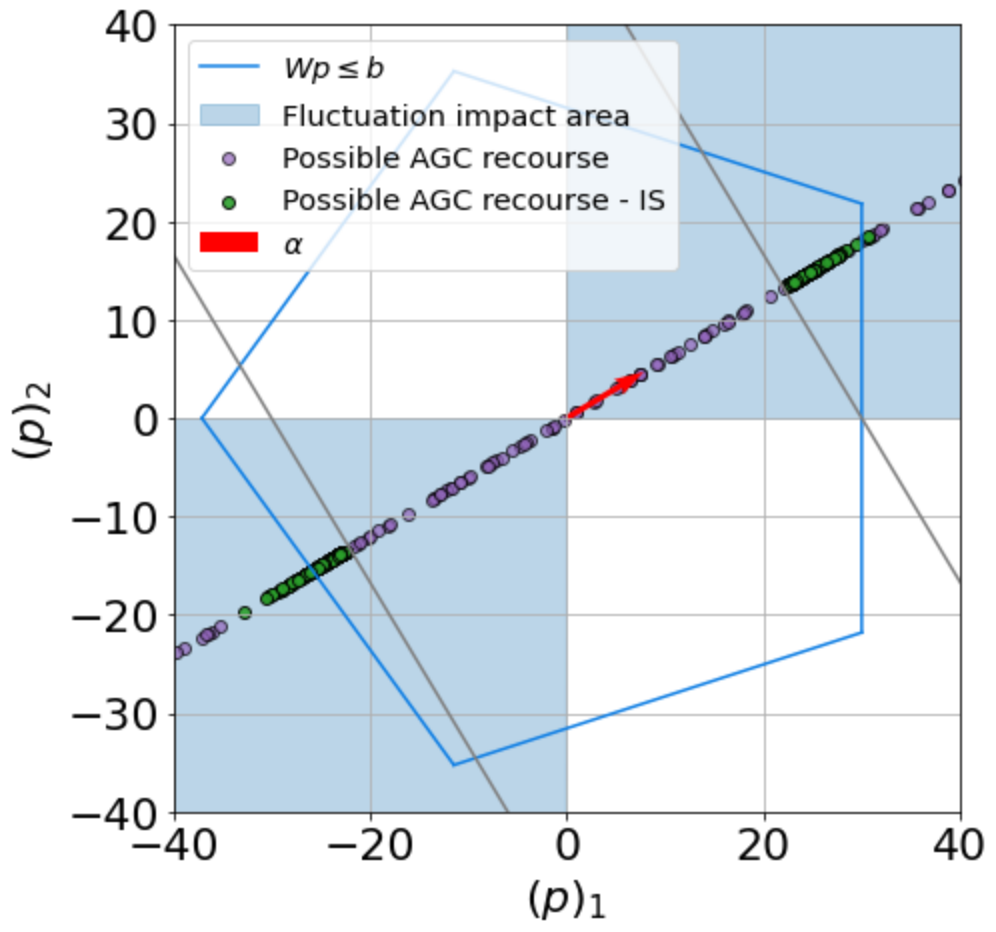
\includegraphics[width=.25\textwidth]{Dissertation/images/dynamic/poly_and_alpha_mc_vs_is.png}
%     \vspace{-5mm}
%     \caption{Realizations of AGC recourse from importance sampling are obtained such that are appear outside of the redundant samples set $\mathcal{P}_r$.
%     }
%     \label{fig:importance_sampled_vs_mc}
%     \vspace{-5mm}
% \end{figure}
 

% \subsection{Numerical Method}\label{sec:nm}
%\vspace{-1mm}
\section{Empirical Study}\label{sec:emp}
%\vspace{-1mm}
\subsection{Algorithms and Implementation Details}
%\vspace{-1mm}
We compare the performance of SA based on different strategies: classical Monte-Carlo (SA) and the proposed A-priori Reduced (AR-SA), and %. Moreover we compare the method proposed with 
the state-of-the-art scenario reduction methods: Fast-Forward, Simultaneous Backward \cite{heitsch2003scenario, dupavcova2003scenario} and K-Means \cite{keutchayan2023problem}. 
Data-Driven Chance Constrained Optimization over Wasserstein Balls (DD-DRO) from \cite{chen2024data}. 
For our test cases, we consider power systems from MATPOWER \cite{zimmerman2010matpower}, specifically Grid-6WW \cite{wood2013power} (pp. 104, 112, 119, 123-124, 549), Washington-14 and IEEE-30.
%
We implemented the algorithms using Python 3.9.13 and PandaPower 2.8.0 \cite{pandapower.2018} on a MacBook Pro (M1 MAX, 64 GB RAM). The optimization problems were solved using the Pyomo framework \cite{hart2017pyomo}
%and MindtPy \cite{bernal2018mixed}
, which employed GLPK \cite{Oki2012GLPKL}.% for mixed-integer programs and Ipopt \cite{wachter2006implementation} for non-linear subproblems. Without integer variables were present, MindtPy used only Ipopt. 
%The code is available on GitHub\footnote{https://github.com/vjugor1/OptimalControlScenarioApproximation}.
During the first case study, we reveal that DD-DRO, comparing with classical SA and proposed AR-SA, turns out to able to provide feasible solutions for JCC for fewer number of data samples. However, it is significantly heavier in terms of computation burden and less stable making this method less practical due to its internal complexity.
During the second case study, we compare AR-SA with classical SA and show significant (up to 2 times) improvements in the amount of data samples required to provide reliable solution.

We implemented the algorithms using Python 3.9.13 and PandaPower 2.8.0 \cite{pandapower.2018} on a MacBook Pro (M1 MAX, 64 GB RAM). For solving the optimization problem, we utilized Pyomo framework \cite{hart2017pyomo} and Mixed-Integer Nonlinear Decomposition Toolbox in Pyomo (MindtPy)   \cite{bernal2018mixed} optimization solver, which used GLPK \cite{Oki2012GLPKL} for internal mixed integer programs and Ipopt \cite{wachter2006implementation} for internal non-linear subproblems. MindyPy automatically detects if the problem provided does not have integer variables (SA and AR-SA cases) and uses Ipopt solely. 
The code for this chapter is available on Github\footnote{https://github.com/vjugor1/OptimalControlScenarioApproximation}.
%\vspace{-4mm}
\subsection{Test Cases and Numerical Results}
%\vspace{-1mm}
We conducted three case studies to evaluate the performance of SA, AR-SA, and other scenario reduction methods under different scenarios.  The first study focuses on the Grid-6WW and Washington-14, comparing the number of samples $N$ needed to achieve the $1-\rho=0.99$ reliability of $1-\eta$ feasible solution among 5 methods. 
The second study analyzed IEEE-30 bus system, which consist of 30 buses. 
In this case, we compared the number of samples needed to achieve a solution reliability of $1-\rho=0.99$ and assessed the total execution time, including the scenario reduction step. We summarized the required number of samples in Table \ref{tab:summary_results}. The value of $1-\eta$ is given by out-of-sample Monte Carlo; the empirical reliability is given by averaging over $L=100$ independent CC-OPF problem instances, as described in Algorithm~\ref{alg:estimate_delta}.
%
In all case studies, we model power generation and consumption fluctuations with a standard deviation of 0.01 of their nominal values, increasing cumulatively for each temporal snapshot. Thus, we expressed fluctuations as $\xi^t \sim \mathcal{N}(0, (\tilde{\sigma_t}^2))$, where $\tilde{\sigma_t}^2 = \tilde{\sigma}_0^2 \cdot t$. Simulations were carried out over $T=3$ temporal snapshots.% for each test case.
The third one compares SA, AR-SA and DD-DRO on Grid-6WW by estimating produced solutions' reliability and execution time.
The evaluation between SA, AR-SA, DD-DRO aims at a comparison of the number of samples $N$ required to obtain a solution with a reliability of $1-\rho$ (feasible for Problem \eqref{eq:optimal_control_2} with prob. $1-\rho$) and total execution time. Since DD-DRO is solved via complex mixed-integer non-linear programming \cite{chen2024data}, it is important to compare execution time together with amount of data required.
The second case study seeks to compare AR-SA and classical SA in the number of samples $N$ required to obtain a solution with a reliability of $1-\rho$.% As explained in Section \ref{sec:chancecontrol}, $1 - \eta$ stands for the confidence threshold for linear constraints, and $1-\rho$ is the probability of the scenario approximation solution to be feasible for.

\paragraph{Evaluation methodology.}
To get an empirical estimation of the solution reliability $1-\hat{\rho}$, we independently construct $L=100$ different approximations for both  SA and reduced SA. Further, we shortname SA with scenarios reduced by FF, SB and K-Means and $\hat{\mathcal{P}}_r$ as SA-FF, SA-SB, SA-KMeans and AR-SA respectively. The data-driven approximation size $N$ starts with $3$ and increases until the corresponding scenario approximation problem reaches $1-\hat{\rho} > 0.99$. For each approximation, we obtain $L$ different solutions: $(x^*_N)_l, ~ l=1, \dots, L$. We estimate the confidence of each obtained solution by running a series of out-of-sample validations. We use $10^4$ Monte-Carlo samples of $\xi$ to estimate of JCC feasibility constraint $(\hat{\mathbb{P}}_N)_l$, $l=1, \dots, L$. Finally, the solution reliability is given by $1 - \hat{\rho}$. It represents the fraction of $L$ solutions $(x^*_N)_l$ such that $(\hat{\mathbb{P}}_N)_l \geq 1 - \eta$. 
Alg.~\ref{alg:estimate_delta} summarizes the sequence of steps.

\begin{algorithm}[ht]
\SetKwInOut{Input}{input}
\SetKwRepeat{Do}{do}{while}
% \SetKwInOut{Output}{output}
\caption{Reliability $1-\hat{\delta}$ -- an empirical estimate}\label{alg:estimate_delta}
\Input{$L$ -- number of trials, DC-OPF problem parameters, $\eta$ -- confidence level, $N_0$ -- initial size of scenario approximation, $N_{\max}$ -- maximal size of scenario approximation}
$N \gets N_0$\;
$\hat{ \boldsymbol \delta}$ -- storage for $\hat{\delta}_N$\;
\Do{$N \leq N_{\max}$}
{
     $C_N \gets 0$ -- feasibility counter\;
     $l \gets 1$\;
    \Do{$l \leq L$}{
        Obtain $(x^*_N)_l$ -- scenario approximation with $N$ samples (using SA-IS or SA) \;
        Estimate constraint satisfaction probability $(\hat{\mathbb{P}}_N)_l$ using Monte Carlo samples.\label{alg:estimate_delta:phat_N_l}\;
        \uIf{$(\hat{\mathbb{P}}_N)_l \geq 1 - \eta$}{
            $C_N \gets C_N +1$
        }
        }
    $1-\hat{\delta}_N \gets C_N / L$ -- fraction of trials turned out to be feasible \;
    Append $\hat{\delta}_N$ to $\hat{ \boldsymbol \delta}$ \;
    $n  \gets n + N_{\max}/ 10$\;
}
\Return $\hat{ \boldsymbol \delta}$
\end{algorithm}

\paragraph{Complexity and Execution Time}
In addition to solving the SA optimization problem of type \eqref{eq:optimal_control_sampling_02}, selecting scenarios requires computational effort. The complexity of standard Monte Carlo-based SA (denoted as SA) does not require scenario reduction, unlike other methods, which need additional computations.

The Fast Forward method adds scenarios one by one based on probabilistic metrics (2-Wasserstein distance) and redistributes probabilities after each addition. Simultaneous Backward, on the other hand, removes scenarios using the same process. Denoting $N_r$ as the target number of scenarios after reduction, the complexities of these methods are $O(N_r^3 + N_r N^2)$ and $O(N_r^3 + N^3)$, respectively \cite{heitsch2003scenario, rujeerapaiboon2022scenario}. The K-Means algorithm is based on iterative estimation of scenario cluster centers and requires estimation of $L_2$ distance between scenarios and cluster centers. This algorithm requires $O(N_rN^2)$ \cite{pakhira2014linear} operations. Contrary, in the proposed AR-SA the reduction step is conducted via checking if a current samples is within $\hat{\mathcal{P}}_r$, thus, the complexity is $O(N)$. The construction of $\hat{\mathcal{P}}_r$ itself grows linearly with the number of deterministic constraints under probability measure in JCC of \eqref{eq:optimal_control_2}. 

We analyze the implications of the computational complexity by measuring total execution time: reduction and solving corresponding reduced scenario approximation. We conducted this experiment on IEEE-30 grid with target JCC feasibility level of $1-\eta=0.99$. The results are shown in Figure \ref{fig:ieee30time}. Here one can observe that the execution time almost similar for all the reduction methods with classical Monte-Carlo SA, except SA-SB. This indicates that the scenario reduction is computationally cheap operation, in comparison with solving optimization problem. Also, this experiment supports the proposed method in tractability.

% We consider the grid constraints to be satisfied with probability $1-\eta = 0.9$. The parameters for DD-DRO are as follows: Wasserstein ball with radius $r_W = 10^{-3}$, maximum function relaxation constant $M = 10$. Such parameters are chosen as minimal for $\eta$ and maximal for $r_W$ as possible, since for smaller $\eta$ and larger $r_W$ feasibility set of the DD-DRO turned out to be empty which was reported by the solver. The latter hints on an excessive conservativeness of the DD-DRO approach. Within non-strict reliability setup ($\eta=0.1$) we compare three methods: DD-DRO, SA and proposed AR-SA. We used the same number of samples for these methods, DD-DRO was based on the same samples that were used for classical SA, since changing the removing samples as proposed for AR-SA ones changes the underlying distribution of data and corrupts ambiguity set of DD-DRO. We were solving the corresponding optimization problem for $L=100$ independently sampled datasets.
%
%Figures \ref{fig:grid6reliability} and \ref{fig:grid6time} compare the performance of three methods on reliability and execution time. From the first figure, one can observe that DD-DRO, even for 2 data samples is able to produce solution that is more reliable for the original JCC Problem \ref{eq:optimal_control_2}. However, the boxplots that were produced from the reliabilities of DD-DRO solution are significantly more spread than of the SA and AR-SA, indicating method's instability. Also, average execution time of DD-DRO is uniformly five times larger than those of SA and AR-SA. The latter is caused by the fact that the underlying problem is non-linear and contains binary variables. In addition, DD-DRO optimization problem requires to assign 2 variables (1 binary and 1 positive real) for each data sample. Specifically, for Grid-6WW case with $N=100$ data samples, DD-DRO has 205 variables with 100 binary among them and 16302 constraints. Meanwhile, SA and AR-SA have only 4 continuous variables and 16203 constraints. 
%
Having conducted this analysis, we continue with SA and AR-SA and other reduction methods on larger grids and more strict reliability ($\eta = 0.05, ~0.01$) requirements in JCC optimization problem \eqref{eq:optimal_control_2}.
\vspace{-1mm}
\paragraph{ SA Solution Reliability.}
\begin{table}[t]
\caption{The number of samples for AR-SA and SA required in CC-OPF with a confidence threshold of $1-\eta$ to get the empirical reliability of $1-\hat{\rho} = 0.99$. 
    }
    \centering
    % \adjustbox{width=\linewidth}{
        % \begin{tabular}{lrr|lr|ll}
        \begin{tabular}{|lr|rlrll|}
        \toprule
        Case & $\eta$ & SA & AR-SA & SA-FF & SA-SB & SA-KMeans \\
\midrule
grid14 & 0.05 & 93 & 48 & 48 & 138 & 48 \\
grid30 & 0.05 & 138 & 93 & 138 & 138 & 93 \\
grid14 & 0.01 & 363 & 93 & 363 & 363 & 363 \\
grid30 & 0.01 & 453 & 273 & 453 & 453 & 453 \\
\bottomrule
  % Case &  $\eta$ &  SA No &             SA Cost &  AR-SA No &          AR-SA Cost & DC-OPF Cost \\
  %       \midrule
  %           grid14 &    0.05 &     93 & 5.5e+03$\pm$1.2e-11 &        48 & 5.5e+03$\pm$5.5e-12 &     5.2e+03 \\
  %           grid30 &    0.05 &     273 & 6.0e+03$\pm$2.8e-11 &        93 & 6.3e+03$\pm$1.3e-11 &     5.7e+03 \\
  %           grid14 &    0.01 &    273 & 5.6e+03$\pm$1.5e-11 &        93 & 5.5e+03$\pm$1.5e-11 &     5.2e+03 \\
  %           grid30 &    0.01 &    363 & 6.2e+03$\pm$4.5e-12 &       183 & 6.1e+03$\pm$4.5e-12 &     5.7e+03 \\
  %           \bottomrule
        \end{tabular}
    % }
    \label{tab:summary_results}
\end{table}
Following this analysis, we evaluate methods on larger grids with high reliability requirements. % ($\eta = 0.05, ~0.01$) for the JCC optimization problem \eqref{eq:optimal_control_2}.
%We analyse of numerical performance of classical SA and proposed AR-SA in more details over large test cases. 
This experiment seeks to find the number of samples sufficient for a solution of data-driven approximation to be feasible for original JCC with high probability for different $\eta$.
We estimate the number of samples required to reach confidence thresholds of $1-\eta = 0.95$ and $0.99$ with reliability of $0.99$ for AR-SA, SA, SA-FF, SA-SB and SA-KMeans in Table~\ref{tab:summary_results}, showing the number of samples required is 30-50\% less for AR-SA compared to classical SA and the advantage of AR-SA increases with the increase of $1-\eta$.

\begin{figure}[hbt]
    \centering
    \begin{subfigure}{.9\textwidth}
      \centering
      % include second image
      \hspace{-0mm}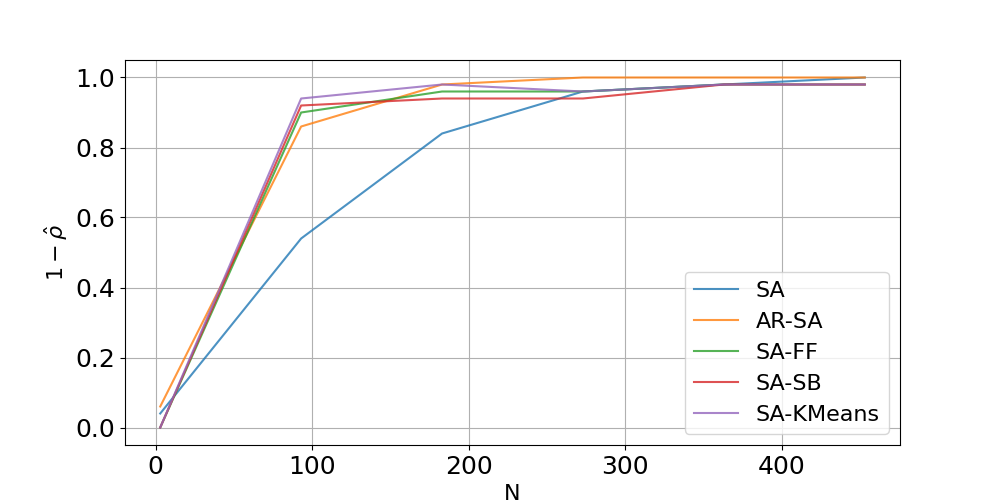
\includegraphics[width=0.99\linewidth]{Dissertation/images/dynamic/ieee30/1_beta_N_453_eta_0.01.png}
      \caption{Empirical reliability %($1-\hat{\rho}$) 
      vs $\#$ samples  in CC-OPF, $\eta = 0.01$.}
      \label{fig:ieee30conservatism}
    \end{subfigure}\\
        
    \begin{subfigure}{.9\textwidth}
      \centering
\hspace{10mm}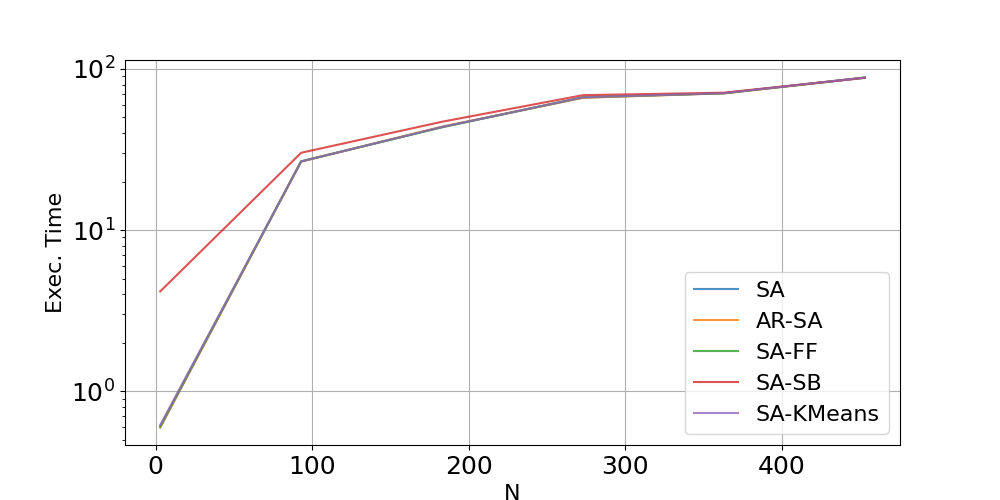
\includegraphics[width=0.99\linewidth]{Dissertation/images/dynamic/ieee30/exec_time_N_453_eta_0.01.png}~~~~~~\hfill
      \caption{Exec. time vs $\#$ samples, $\eta = 0.01$.
      }
      \label{fig:ieee30time}
    \end{subfigure}
    \caption{Numerical comparison of execution time and the reliability of reduced approximations' solution on IEEE 30 bus system.  
    }
\label{fig:ar-sa-ieee30}
\end{figure}

\begin{figure}[hbt]
    \centering
    \begin{subfigure}{.9\textwidth}
      \centering
      % include second image
      \hspace{-0mm}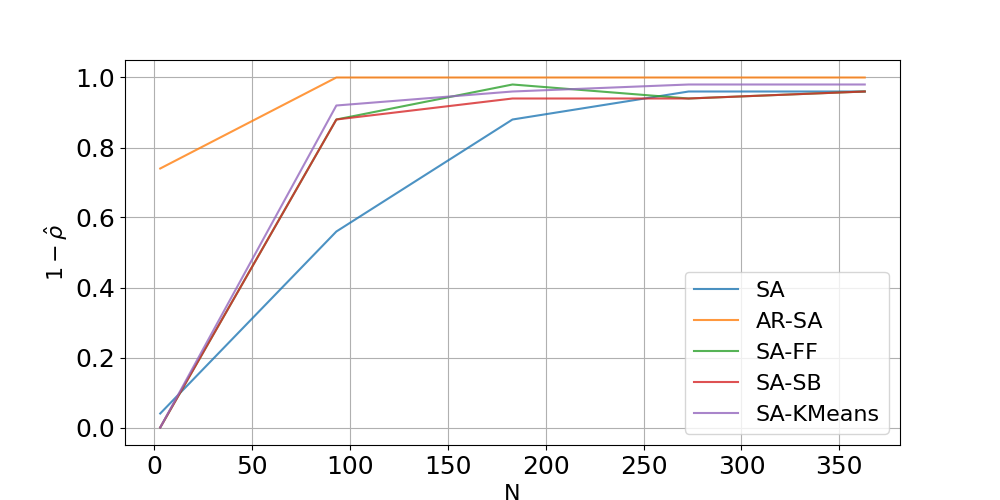
\includegraphics[width=0.99\linewidth]{Dissertation/images/dynamic/washington14/1_beta_N_363_eta_0.01.png}
      \caption{Washington 14 bus, $\eta = 0.01$.}
      \label{fig:washington14conservatism}
    \end{subfigure}
    
    \begin{subfigure}{.9\textwidth}
      \centering
      % include second image
      \hspace{0mm}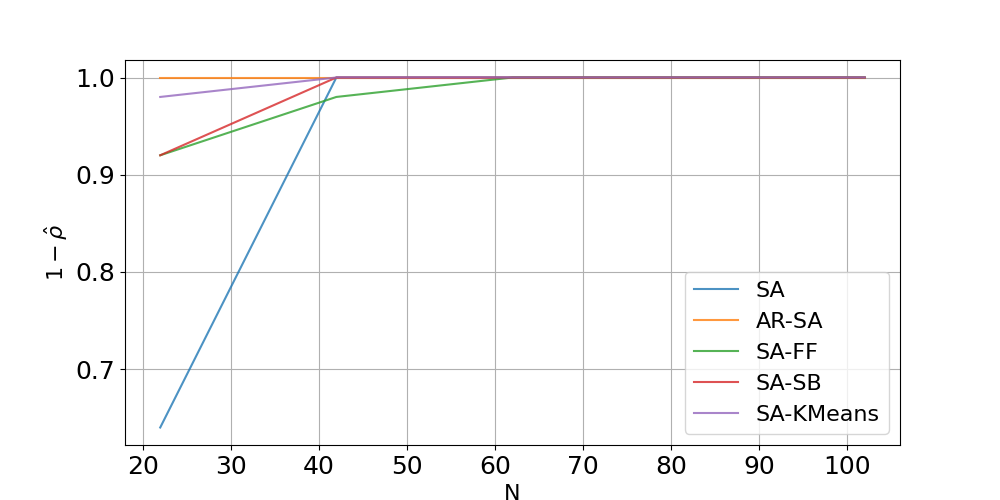
\includegraphics[width=0.99\linewidth]{Dissertation/images/dynamic/grid6/1_beta_N_102_eta_0.1.png}
      \caption{Grid6-WW 6 bus system, $\eta = 0.1$.}
      \label{fig:grid6reliability}
    \end{subfigure}
    \caption{Numerical comparison of reduced approximations' solution: empirical reliability ($1-\hat{\rho}$) vs $\#$ samples for CC-OPF.  
    }
\label{fig:ar-sa-wash14-grid6}
\end{figure}

\begin{figure}[hbt]
    \centering
    \begin{subfigure}{.9\textwidth}
      \centering
      % include second image
      \hspace{0mm}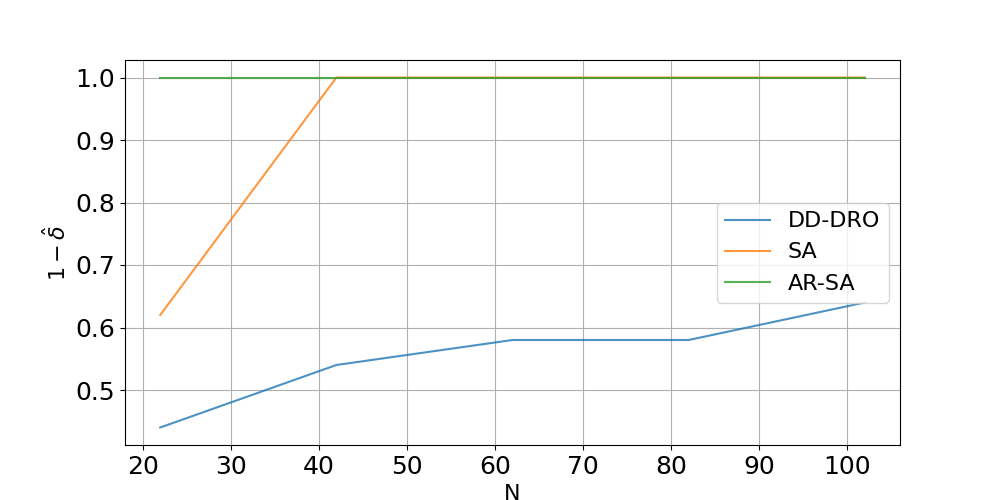
\includegraphics[width=0.99\linewidth]{Dissertation/images/dynamic/grid6/dd-dro/1_beta_N_102_eta_0.1.png}
      \hspace{0mm}\caption{Empirical reliability %($1-\hat{\rho}$) 
      vs $\#$ samples in CC-OPF, $\eta = 0.1$.}
      \label{fig:grid6reliability-dd-dro}
    \end{subfigure}
    
    \begin{subfigure}{.9\textwidth}
      \centering \hspace{10mm}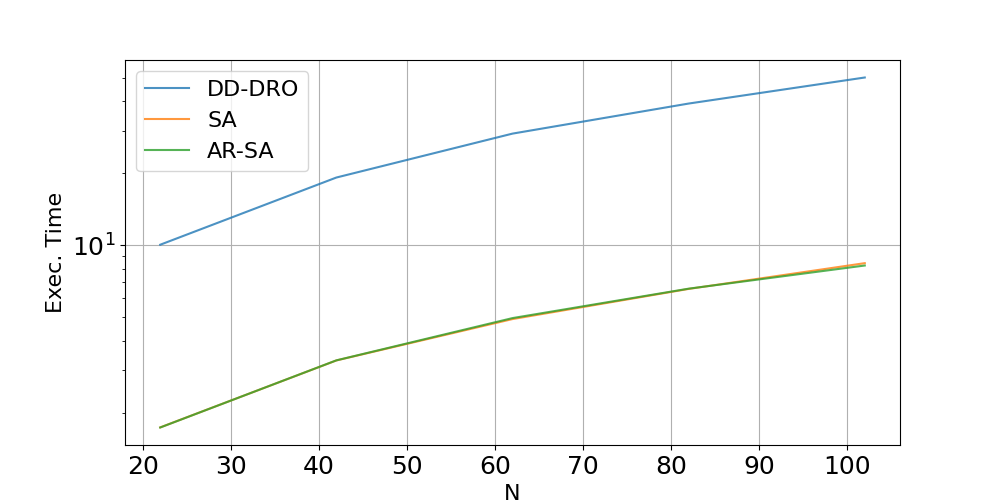
\includegraphics[width=0.99\linewidth]{Dissertation/images/dynamic/grid6/dd-dro/exec_time_N_102_eta_0.1.png}~~~~~~\hfill
      \caption{Exec. time vs $\#$ samples, $\eta = 0.1$.
      }
      \label{fig:grid6time-dd-dro}
    \end{subfigure}
    \caption{Numerical comparison of execution time and the reliability between classical MC based SA, AR-SA and DD-DRO on Grid6-WW 6 bus system.  
    }
\label{fig:ar-sa-vs-dd-dro}
\end{figure}

\begin{comment}
\begin{figure*}[hbt]
\vspace{-3mm}
\vspace{-3mm}
% \begin{subfigure}{.5\textwidth}
%   \centering
%   % include second image
%   \hspace{-1mm}\includegraphics[width=\linewidth]{Dissertation/images/dynamic/ieee57/1_beta_N_633_eta_0.01.png}
%   \caption{Empirical reliability $(1-\hat{\rho})$ versus the number of samples $N$\\ in CC-OPF for IEEE 57 bus system, $\eta = 0.01$.}
%   \label{fig:ieee57conservatism}
% \end{subfigure}
% \begin{subfigure}{.5\textwidth}
%   \centering
%   % include first image
%   \includegraphics[width=\linewidth]{Dissertation/images/dynamic/ieee57/boxplot_J_N_633_eta_0.01.png}~~~~~~\hfill
%   \caption{Spread of the probability of constraint feasibility, $(\hat{\mathbb{P}}_N)_l$, versus number of samples $N$ in CC-OPF for IEEE 57 bus system, $\eta = 0.01$.}
%   \label{fig:ieee57reliability}
% \end{subfigure}
\begin{subfigure}{.5\textwidth}
  \centering
  % include second image
  \hspace{-1mm}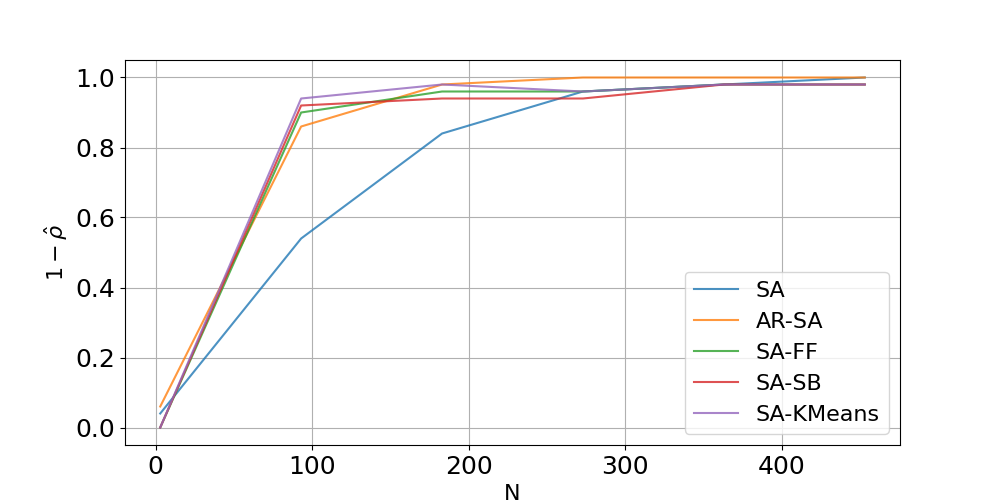
\includegraphics[width=\linewidth]{Dissertation/images/dynamic/ieee30/1_beta_N_453_eta_0.01.png}
  \caption{Empirical reliability ($1-\hat{\rho}$) versus number of samples $N$ \\ in CC-OPF for IEEE 30 bus system, $\eta = 0.01$.}
  \label{fig:ieee30conservatism}
\end{subfigure}
\begin{subfigure}{.5\textwidth}
  \centering
  % include first image
  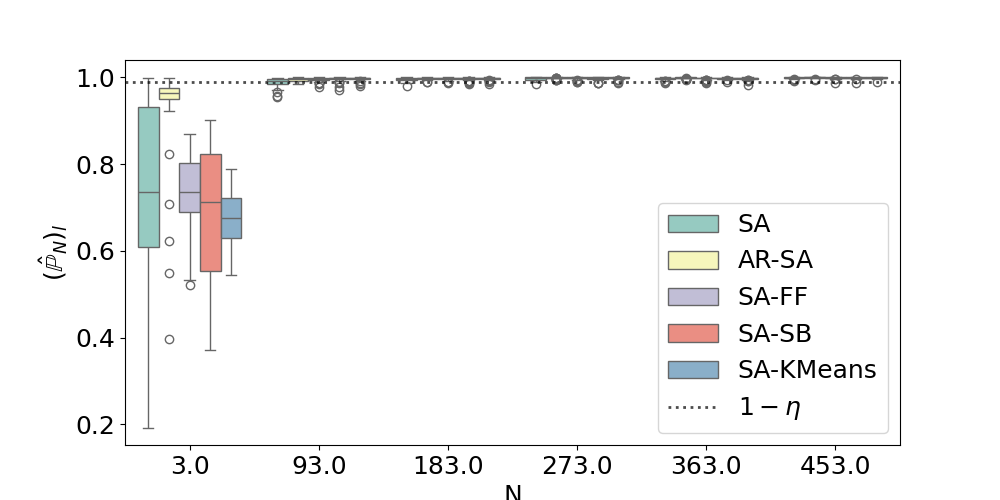
\includegraphics[width=\linewidth]{Dissertation/images/dynamic/ieee30/boxplot_J_N_453_eta_0.01.png}~~~~~~\hfill
  \caption{Spread of the probability of constraint feasibility, $(\hat{\mathbb{P}}_N)_l$, versus the number $N$  of samples in CC-OPF for IEEE 30 bus system, $\eta = 0.01$.}
  \label{fig:ieee30reliability}
\end{subfigure}
% \begin{subfigure}{.5\textwidth}
%   \centering
%   % include second image
%   \hspace{-1mm}\includegraphics[width=\linewidth]{Dissertation/images/dynamic/washington14/1_beta_N_633_eta_0.01.png}
%   \caption{Empirical reliability ($1-\hat{\rho}$) versus number of samples $N$ \\ in CC-OPF for Washington 14 bus system, $\eta = 0.01$.\\}
%   \label{fig:washington14conservatism}
% \end{subfigure}
% \begin{subfigure}{.5\textwidth}
%   \centering
%   % include first image
%   \includegraphics[width=\linewidth]{Dissertation/images/dynamic/washington14/boxplot_J_N_633_eta_0.01.png}~~~~~~\hfill
%   \caption{Spread of the probability of constraint feasibility, $(\hat{\mathbb{P}}_N)_l$, versus the number $N$ of samples in CC-OPF for the Washington case, $\eta = 0.01$.}
%   \label{fig:washington14reliability}
% \end{subfigure}
\vspace{-2mm}
\caption{(a) Empirical reliability ($1-\hat{\rho}$) and (b) The spread of constraint feasibility $(\hat{\mathbb{P}}_N)_l$ for CC-OPF ($1-\eta =.99$) in IEEE 57 \& 30 bus, the Washington 14 resp. system. The three cases correspond to samples in CC-OPF drawn from SA and AR-SA. The empirical estimates are computed with $L = 200$ optimization instances (for $1-\hat{\rho}$), and $N_{MC}=10^4$ Monte-Carlo samples for each instance to determine constraint validation (for box-plot of $(\hat{\mathbb{P}}_N)_l$), as described in Algorithm~\ref{alg:estimate_delta}. 
Colored boxes stand for the 25\% -- 75\% interquartile range (IQR). Diamonds show samples outside of the $\pm 1.5*\text{IQR}$. 
Note that both in reliability and the IRQ of constraint feasibility, AR-SA requires much less number of samples compared to SA or~SA-O.}
\label{fig:ieee118}
\end{figure*}
\end{comment}
%To better illustrate the dependency between number of samples in the approximation $N$ and relibaility estimates $1 - \hat{\rho}$, we demonstrate Figure \ref{fig:ieee30reliability}.
We illustrate the dependence between empirical reliability, $1-\hat{\rho}$, and the number of samples, $N$, for different values across the IEEE-30, Washington-14 and Grid6-WW systems in Figures \ref{fig:ar-sa-wash14-grid6} and \ref{fig:ar-sa-wash14-grid6}. Here, Figures \ref{fig:ieee30conservatism}, \ref{fig:washington14conservatism}, \ref{fig:grid6reliability} illustrate empirical reliability ($1-\hat{\rho}$), meanwhile Figures \ref{fig:ieee30time}, \ref{fig:grid6time-dd-dro} -- Execution time for various power grid test cases. The empirical estimates are computed with $L = 100$ optimization instances (for $1-\hat{\rho}$), and $N_{MC}=10^4$ Monte-Carlo samples for each instance to determine constraint validation (for box-plot of $(\hat{\mathbb{P}}_N)_l$), as described in Algorithm~\ref{alg:estimate_delta}. We maintain a confidence threshold for JCC feasibility of $1-\eta = 0.99$. 
Also, we present box plots showing the spread of $(\hat{\mathbb{P}}_N)_l$—the empirically computed probability of constraint satisfaction using $10^4$ Monte Carlo samples as per Algorithm \ref{alg:estimate_delta}, see Eq.~\ref{alg:estimate_delta:phat_N_l}. 
Notably, AR-SA achieves higher reliability levels ($1-\hat{\rho}$) with significantly fewer samples $N$. From Figures \ref{fig:ieee30conservatism},  \ref{fig:washington14conservatism} and \ref{fig:grid6reliability} one can observe that for Washington-14 and Grid6-WW AR-SA reaches high reliability levels with a lower number of samples and in IEEE-30 case, though SA, SA-FF, SA-SB, and SA-KMeans reach $1 - \rho = 0.9$ with less samples, the higher $1 - \rho =0.99$ reliability level is reached by AR-SA first. This observation is due to the problem-specific redundancy set $\hat{\mathcal{P}}_r$ construction that is able to filter specifically those scenarios that are irrelevant for the given problem.

\paragraph{AR-SA and DD-DRO comparison.}
We assessed grid constraints to be met with a probability of $1-\eta = 0.9$. For DD-DRO, we set the parameters as follows: a Wasserstein ball radius of $r_W = 10^{-3}$ and a maximum function relaxation constant of $M = 10$. These parameters were selected to be minimally conservative for $\eta$ and maximally expansive for $r_W$, as smaller $\eta$ values and larger $r_W$ values led to an empty feasibility set, indicating excessive conservativeness of DD-DRO. In a non-strict reliability setup ($\eta=0.1$), we compared DD-DRO, SA, and the proposed AR-SA using an identical number of samples. For DD-DRO, we use the same sample set as for classical SA to prevent changes in the underlying data distribution that would affect the ambiguity set of DD-DRO when adopting the sample reduction strategy for AR-SA. Figures \ref{fig:grid6reliability-dd-dro} and \ref{fig:grid6time-dd-dro} illustrate the performance differences in reliability and execution time across methods. Notably, DD-DRO achieved higher reliability for the JCC Problem \eqref{eq:optimal_control_2} even with just two data samples. But, its reliability boxplots were significantly more spread than those of SA and AR-SA, indicating instability. The average run time for DD-DRO is consistently 5x longer than that for SA and AR-SA, owing to the non-linear nature of the problem and the inclusion of binary variables. Indeed, in the Grid-6WW case with $N=100$ data samples, DD-DRO handle 205 variables, including 100 binary, and 16,302 constraints, while SA and AR-SA use only 4 continuous variables and 16,203 constraints.
%The box plots reveal that AR-SA rapidly reduces the variance in the solutions’ chance-constraint feasibility, characterized by thinner box plots and fewer outliers, compared to SA.
%We illustrate the dependence between empirical reliability $1-\hat{\rho}$ and $N$ over a range of values for the IEEE-30 (Washington-14) bus system in Fig.~ \ref{fig:ieee30reliability} (\ref{fig:washington14reliability}). Here, we keep a confidence threshold of joint chance constraint feasibility $1-\eta =0.99$. Moreover, we present box-plots for the spread of $(\hat{\mathbb{P}}_N)_l$ for different $N$, in Fig.~\ref{fig:ieee30conservatism} (\ref{fig:washington14conservatism}). We denote $(\hat{\mathbb{P}}_N)_l$ as the probability of constraint satisfaction, empirically computed using $10^4$ Monte Carlo samples of Algorithm \ref{alg:estimate_delta}, see Eq.~\ref{alg:estimate_delta:phat_N_l}. Note that AR-SA reaches a higher reliability level ($1-\hat{\rho}$) with a substantially fewer number of samples $N$. These boxplots indicate that the variance in the obtained solution's chance-constraint feasibility reduces faster for AR-SA, noted by thinner boxplots and lack of outliers, compared to SA.
%\vspace{-3mm}
%\begin{figure}[!ht]
    %\centering
    %\vspace{-3mm}
    %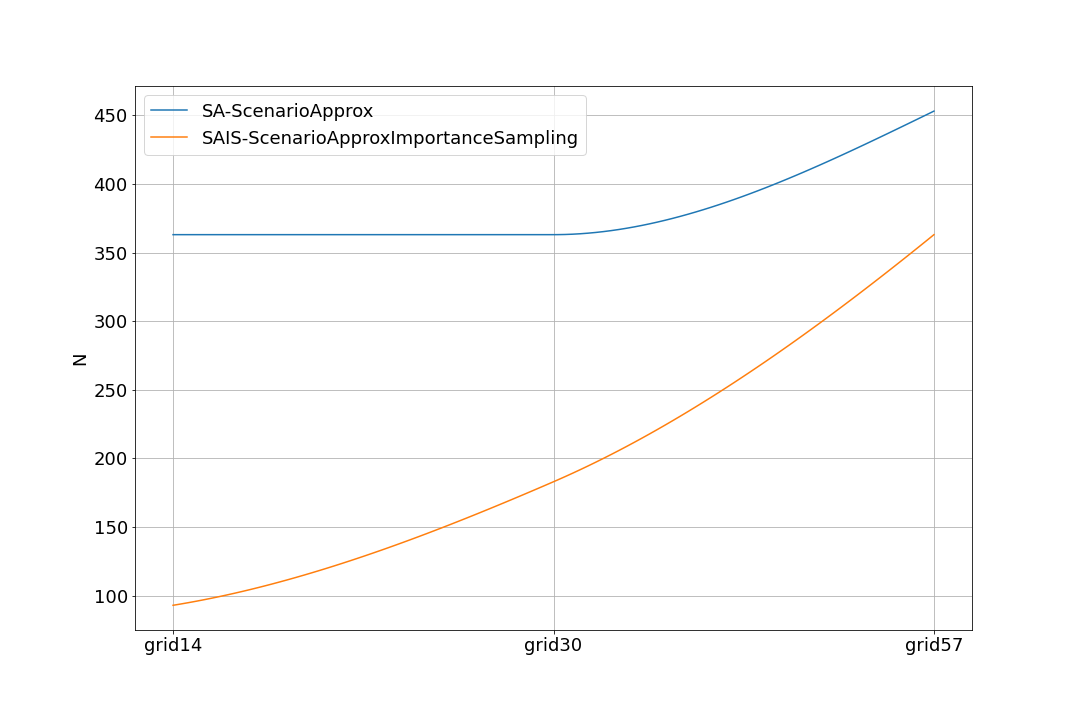
\includegraphics[width=.45\textwidth]{Dissertation/images/dynamic/summary_plot_001.png}
%    \vspace{-5mm}
%    \caption{Number of samples required to reach $0.99$ reliability level depending on the grid case.
%    }
%    \label{fig:summary grid 001}
    %\vspace{-5mm}
%\end{figure}

%Figure~\ref{fig:summary grid 001} illustrates the superior sample efficiency of AR-SA.
% \vspace{-1mm}
\section{Conclusion}\label{sec:conclusion}
% \vspace{-1mm}
Data-driven approximations are useful in chance-constrained stochastic programs with unknown uncertainty distribution and/or JCC settings. However, the data requirements rapidly become infeasible with the increase in size and reliability requirements. To address this, we proposed a novel approach that allows us to a-priorily identify and remove redundant scenarios in stochastic approximations for JCC dynamic multi-timestamp DC-OPF. We prove the validity of this approach theoretically and 
ensured its high empirical performance over various test cases. 